\documentclass[a4j, twocolumn, dvipdfmx]{jsarticle}  % 研究計画は1段組が読みやすい（日本語対応）

\usepackage[a4paper, left=2.0cm, right=2.0cm, top=2.0cm, bottom=2.0cm]{geometry} % 余白を標準寄りに
\usepackage{amsmath}   % 数式用
\usepackage[dvipdfmx]{graphicx}
\usepackage{titlesec}  % 見出し調整
\usepackage{enumitem}  % 箇条書きの余白調整（見やすさ改善）
\usepackage{tikz}
\usetikzlibrary{positioning}
\usepackage{algorithm}
\usepackage{algpseudocode}
\usepackage{float}
\usepackage{flushend}  % 最終ページの左右コラムの高さを自動でそろえる（余白の偏り対策）

% =========================================================
% 見出し設定
% =========================================================
\titleformat{\section}[block]
  {\normalfont\large\bfseries}
  {\thesection}{0.7em}{}

\titleformat{\subsection}[block]
  {\normalfont\normalsize\bfseries}
  {\thesubsection}{0.7em}{}

\titleformat{\subsubsection}[block]
  {\normalfont\normalsize\bfseries}
  {\thesubsubsection}{0.7em}{}

% 見出し前後の余白
\titlespacing*{\section}
  {0pt}{1.5ex plus 0.5ex minus 0.2ex}{0.8ex}

\titlespacing*{\subsection}
  {0pt}{1.2ex plus 0.4ex minus 0.2ex}{0.6ex}

% =========================================================
% 箇条書き設定
% =========================================================
\setlist[itemize]{
  topsep=3pt,
  itemsep=1pt,
  parsep=0pt,
  leftmargin=*
}


% 箇条書きの詰まりを軽減
\setlist[itemize]{topsep=4pt, itemsep=2pt, leftmargin=*}

\title{
Federated LearningにおけるAdaptive Model Poisoning AttackとRobust Aggregationの評価に関する実験
}
\author{3CDA2216 笠原秀星}
\date{\today}

\begin{document}

\maketitle  % タイトルを表示

\section{研究背景・概要}

Federated Learning（以下, FL）は, 生データを共有することなく複数のデバイスや組織が協調して機械学習モデルを学習する分散学習の枠組みである\cite{mammen2021fl}.
FLは, ユーザのプライバシー保護と機械学習の両立を可能にする技術として注目されており, スマートフォンにおける単語予測や顔認識, 音声認識技術の向上に利用されている. また, 厳格なプライバシー規制によりデータ共有が困難な医療分野や, 自動運転車におけるリアルタイムデータの活用など, 幅広い分野への応用が期待されている\cite{li2019fl}.

一方で, FLには収束性, データ分布の不均一性（Non-I.I.D.）, 通信コスト, 大規模環境への適用, モデル集約手法など, さまざまな課題が存在する\cite{ma2020privacy}. 特に, FLでは多数の参加者が学習に関与するため, 悪意のあるクライアントによる攻撃への耐性を確保することが重要な研究課題となっている. 医療データや個人情報などの機密性の高いデータを扱う応用が想定されることから, 安全かつ信頼性の高い学習環境の実現が求められている.

FLに対する代表的な攻撃としてPoisoning Attackが挙げられる. Poisoning Attackは大きくData Poisoning AttackとModel Poisoning Attackの2種類に分類される. Data Poisoning Attackは学習データそのものを改ざんする攻撃であり, ラベル反転攻撃やBackdoor Attackなどが含まれる. 一方, Model Poisoning Attackはクライアントがサーバへ送信するモデル更新や勾配情報を改ざんする攻撃であり, 勾配操作や最適化手法を利用した攻撃などが提案されている.

これらの攻撃に対する防御手法としては, 異常検知, Robust Aggregation, 摂動機構の3つに大別される. 異常検知にはコサイン類似度やクラスタリング, スコアベース手法などが用いられる. また, Robust AggregationにはKrum, Trimmed Mean, Median, Bulyanなどの集約手法が提案されている. さらに, 摂動機構としては差分プライバシーを利用した手法が広く研究されている\cite{sagar2023survey}.

本研究では, これらの中でもModel Poisoning Attackに着目する. Data Poisoning Attackに関してはこれまで多くの研究が行われており, 攻撃に対してロバストな集約手法や検知手法が多数提案されている. 一方で, Model Poisoning Attackは学習データではなくモデル更新そのものを改ざんするため, サーバ側から攻撃を識別することが困難であり, より深刻な脅威となる. また, その防御手法に関する研究はData Poisoning Attackと比較して十分に進んでいるとは言えない.

さらに, FangらはAdaptive Model Poisoning Attackを提案し, 既存のRobust Aggregation手法を考慮した攻撃によって防御機構を回避できる可能性を示している\cite{fang2020local}. このことは, 従来の防御手法が必ずしも十分な耐性を有していないことを示唆しており, Adaptive Model Poisoning Attackに対する詳細な評価が必要である.

そこで本研究では, IID環境およびNon-IID環境においてAdaptive Model Poisoning AttackがFLの学習性能に与える影響を評価する. また, KrumやTrimmed MeanなどのRobust Aggregation手法に対する攻撃の有効性を比較・分析し, 既存防御手法の限界を明らかにする. さらに, 攻撃が成立する要因について考察するとともに, Model Poisoning Attackに対する効果的な防御手法について検討することを目的とする.

\section{事前知識}
\subsection{Federated Learning}
%FLとは何か.従来の機械学習とは何が違うのか.どういうアルゴリズムを用いるのかなど基礎的なFLの知識について述べる.
%通信ラウンド,クライアント,サーバ
%FLを攻撃と防御の観点からカテゴリー分けする.
先に述べたようにFederated Learningは生データを共有することなく複数のデバイスや組織が協調して機械学習モデルを学習する分散学習の枠組みである\cite{mammen2021fl}.
集約アルゴリズムとしてFederated Averaging (以下,FedAvg)を用いる.FedAvgはGoogleが2016年に発表した論文の中で示されたものである\cite{mcmahan2017fedavg}.

\subsubsection{FedAvg}
\begin{table}[t]
\centering
\caption{FedAvgで用いる主な記号}
\begin{tabular}{ll}
\hline
記号 & 意味 \\
\hline
$K$ & 全クライアント数 \\
$C$ & 各ラウンドで参加する割合 \\
$S_t$ & ラウンド$t$で選択されたクライアント集合 \\
$w_t$ & グローバルモデル \\
$w_{t+1}^k$ & クライアント$k$が更新したモデル \\
$n_k$ & クライアント$k$のデータ数 \\
$E$ & ローカル学習のエポック数 \\
$B$ & ミニバッチサイズ \\
$\eta$ & 学習率 \\
\hline
\end{tabular}
\label{tab:fedavg_symbol}
\end{table}
\begin{algorithm}[t]
\caption{Federated Averaging (FedAvg)}
\label{alg:fedavg}
\begin{algorithmic}[1]

\State \textbf{Server executes:}
\State Initialize $w_0$

\For{each round $t = 1,2,\ldots$}
    \State $m \leftarrow \max(C \cdot K, 1)$
    \State $S_t \leftarrow$ random set of $m$ clients

    \ForAll{$k \in S_t$ in parallel}
        \State $w_{t+1}^{k} \leftarrow \mathrm{ClientUpdate}(k,w_t)$
    \EndFor

    \State $
    w_{t+1}
    \leftarrow
    \sum_{k \in S_t}
    \frac{n_k}{n_t}
    w_{t+1}^{k}
    $
\EndFor

\Statex
\State \textbf{ClientUpdate}$(k,w)$
\State Split $P_k$ into batches of size $B$

\For{$i=1$ to $E$}
    \For{batch $b \in B$}
        \State $
        w \leftarrow
        w-\eta\nabla\ell(w;b)
        $
    \EndFor
\EndFor

\State \Return $w$ to server

\end{algorithmic}
\end{algorithm}
アルゴリズム\ref{alg:fedavg}にFedAvgの処理手順を示す。

まず，サーバはグローバルモデル $w_0$ を初期化する。
その後，各通信ラウンド $t$ において，全クライアント数 $K$ のうち割合 $C$ に応じた $m$ 個のクライアントをランダムに選択する。
選択されたクライアント集合を $S_t$ とする。

選択された各クライアントは，サーバから受け取ったグローバルモデル $w_t$ を用いてローカル学習を実施する。
各クライアントは自身が保有するデータ集合 $P_k$ をミニバッチサイズ $B$ ごとに分割し，エポック数 $E$ 回の学習を行う。
モデル更新には確率的勾配降下法（SGD）を用い，学習率を $\eta$ とすると，各ミニバッチ $b$ に対して次式によりパラメータを更新する。

\begin{equation}
w \leftarrow w-\eta\nabla \ell(w;b)
\end{equation}

ここで，$\ell(w;b)$ はミニバッチ $b$ に対する損失関数であり，$\nabla \ell(w;b)$ はその勾配を表す。

ローカル学習終了後，各クライアントは更新後のモデル $w_{t+1}^{k}$ をサーバへ送信する。
サーバは受信したモデルを，各クライアントの保有データ数 $n_k$ に応じて重み付け平均することで新たなグローバルモデル $w_{t+1}$ を生成する。

\begin{equation}
w_{t+1}
=
\sum_{k \in S_t}
\frac{n_k}{n_t}
w_{t+1}^{k}
\end{equation}

ただし，

\begin{equation}
n_t=\sum_{k\in S_t}n_k
\end{equation}

である。
この処理を複数ラウンド繰り返すことで，生データを共有することなくグローバルモデルを学習する。
\subsection{Data Poisoning Attack}

Data Poisoning Attackは，攻撃者が学習データそのものを改ざんし，グローバルモデルの性能低下や誤動作を引き起こす攻撃である。Federated Learningでは，各クライアントが保有するローカルデータや学習過程をサーバが直接確認できないため，悪意のあるクライアントが改ざんしたデータを用いて学習を行うことで，モデルに悪影響を与えることが可能である\cite{sagar2023survey}。

Data Poisoning Attackは，Label Flipping Attack，Poisoning Sample Attack，Backdoor Attackなどに分類される。Label Flipping Attackは，学習データのラベルを意図的に別のラベルへ変更する攻撃である。例えば，数字認識タスクにおいて「1」のラベルを「7」に変更して学習させることで，モデルの分類性能を低下させることができる。

Poisoning Sample Attackは，学習データそのものを改ざんする攻撃であり，ノイズの付加や特定のパターンの埋め込みなどによって学習結果を操作する。

一方，Backdoor Attackは，特定のトリガを含む入力に対してのみ誤分類を引き起こす攻撃である。攻撃者はトリガ付きデータを学習データへ混入させることで，通常の入力に対する性能を維持したまま，トリガを含む入力に対してのみ攻撃者が指定したラベルを出力するようモデルを誘導する。そのため，Backdoor Attackは高い攻撃成功率とステルス性を有しており，発見が困難であるという特徴を持つ。

Data Poisoning Attackは実装が比較的容易である一方，異常なデータ分布やラベルの偏りを利用した検知手法によって防御できる場合がある。そのため近年では，学習データではなくモデル更新そのものを改ざんするModel Poisoning Attackに関する研究が盛んに行われている\cite{sagar2023survey}\cite{xie2020dba}\cite{nguyen2022flame}。



\subsection{Model Poisoning Attack}

Model Poisoning Attackは，悪意のあるクライアントがサーバへ送信するモデル更新や勾配情報を改ざんし，グローバルモデルの性能低下や誤動作を引き起こす攻撃である。Data Poisoning Attackが学習データそのものを改ざんするのに対し，Model Poisoning Attackは学習後のモデルパラメータを直接操作する点に特徴がある。そのため，サーバ側から攻撃の有無を判断することが困難であり，Federated Learningにおける深刻な脅威の一つとして注目されている\cite{sagar2023survey}。

Model Poisoning Attackは，Gradient Manipulation，Optimization Methods，Untargeted Attackの3種類に分類される\cite{sagar2023survey}。Gradient Manipulationは，モデル更新の勾配を意図的に操作する攻撃であり，勾配反転（Sign Flipping Attack）やランダムな勾配の挿入などが代表例として知られている。これらの攻撃は，グローバルモデルの収束を妨害し，性能を低下させることを目的とする。

Optimization Methodsは，攻撃効果を最大化するようにモデル更新を最適化する攻撃である。攻撃者は正常なモデル更新との差を小さく保ちながら，攻撃目的を達成するようにモデルを改ざんすることで，異常検知や防御機構による検出を回避する。Backdoor AttackやModel Replacement Attackの多くはこの分類に含まれる。

Untargeted Attackは，特定の入力に対する誤分類ではなく，グローバルモデル全体の性能低下を目的とする攻撃である。攻撃者はモデル更新を大きく改ざんすることで，学習の収束を妨害し，モデルの可用性を低下させる。


\subsection{Robust Aggregation}
%Robust Aggregationとは何で,どんな種類があるのか述べる.数式などもあれば良い.
%Krum,Mean,Trimmed Mean,Median,Bulyanなどについて論文で述べられていたはず.
%それぞれの手法については\subsubsectionで書けばいいと思う.
Robust Aggregationは，悪意のあるクライアントによる異常なモデル更新の影響を軽減することを目的とした集約手法である\cite{sagar2023survey}。従来のFedAvgでは，各クライアントから送信されたモデル更新を重み付き平均によって集約するため，悪意のあるクライアントが極端なモデル更新を送信した場合，グローバルモデルが大きな影響を受ける可能性がある。

この問題に対処するため，Byzantine Fault Toleranceの考え方を取り入れたRobust Aggregationが提案されている。代表的な手法としてMean（FedAvg），Median，Trimmed Mean，Krum，Bulyanなどが知られており，異常なモデル更新を除外または影響を低減しながらグローバルモデルを更新する。

\subsubsection{Mean (FedAvg)}

FedAvgは，Federated Learningにおいて最も広く利用されている集約手法である。各クライアントから送信されたモデル更新を，保有するデータ数に応じて重み付け平均することで新たなグローバルモデルを生成する。

FedAvgは実装が容易で計算コストも低いという利点を持つ一方，異常なモデル更新の影響を受けやすいという欠点がある。そのため，Model Poisoning Attackに対して脆弱であることが知られている。

\subsubsection{Median}

Medianは，各パラメータについて中央値を採用する集約手法である。平均値ではなく中央値を利用することで，極端に大きな値や小さな値の影響を受けにくくなる。

そのため，悪意のあるクライアントが異常なモデル更新を送信した場合でも，その影響を軽減できる。しかし，多数のクライアントが攻撃に参加している場合には性能が低下する可能性がある。

\subsubsection{Trimmed Mean}

Trimmed Meanは，各パラメータについて極端に大きい値と小さい値を一定数除外した後に平均を計算する手法である。

この手法は外れ値の影響を低減できるため，単純な平均よりもModel Poisoning Attackに対してロバストである。一方で，正常なクライアントの更新が除外される場合もあり，学習性能が低下する可能性がある。

\subsubsection{Krum}

Krumは，各クライアントのモデル更新と他のクライアントとの距離を計算し，最も多くのクライアントと類似しているモデル更新を選択する手法である。

平均を取るのではなく，信頼できると判断された単一のモデル更新を採用するため，異常なモデル更新を排除しやすいという特徴を持つ。しかし，クライアント数が増加すると計算コストが大きくなるという課題がある。

\subsubsection{Bulyan}

Bulyanは，KrumとTrimmed Meanを組み合わせた集約手法である。まずKrumを用いて信頼できるモデル更新を選択し，その後Trimmed Meanによって集約を行う。

複数のByzantine攻撃に対して高い耐性を持つことが報告されているが，計算コストが大きく，クライアント数が多い環境では実行時間が増加するという欠点がある。

本研究では，FedAvgを基準手法とし，Median，Trimmed Mean，KrumおよびBulyanをRobust Aggregationとして採用する。また，Adaptive Model Poisoning Attackを適用した場合の攻撃成功率やモデル精度の変化を比較し，各集約手法の有効性を評価する。


%あとでそれぞれの手法の代表論文についても確認して示さなきゃいけないと思うけど,とりあえずはこれで.
%まだ論文を読んでないので必要に応じて収集する.
\section{関連研究}

Subhash Sagarらは，Federated LearningにおけるPoisoning Attackおよび防御手法に関する包括的なサーベイを行っている。彼らは攻撃をData Poisoning AttackとModel Poisoning Attackに分類し，さらに防御手法についてもRobust Aggregationや異常検知手法などの観点から体系的に整理している。また，各攻撃手法および防御手法の特徴や課題を比較し，Federated Learningにおけるセキュリティ研究の方向性を示している\cite{sagar2023survey}.

Minghong Fangらは，Byzantine-robust Federated Learningに対するLocal Model Poisoning Attackを提案した。従来のData Poisoning Attackとは異なり，攻撃者は学習データではなく悪意あるクライアントのモデル更新そのものを操作する。攻撃を最適化問題として定式化することで，Krum，Bulyan，Median，Trimmed MeanといったByzantine-robust Aggregation手法に対しても有効な攻撃を実現し，既存の防御手法が十分ではないことを示した\cite{fang2020local}.

Chulin Xieらは，DBA (Distributed Backdoor Attacks) を提案した。従来のBackdoor Attackでは全ての攻撃者が同一のトリガを学習するのに対し，DBAではグローバルトリガを複数のローカルトリガへ分割し，各悪意あるクライアントへ分散して埋め込む。この手法により，従来手法と比較して高い攻撃成功率とステルス性を実現できることを示した\cite{xie2020dba}.

Eugene Bagdasaryanらは，Model Replacement Attackを提案した。この攻撃では，攻撃者が生成した悪意あるモデル更新を拡大して送信することで，集約後のグローバルモデルへBackdoorを埋め込むことが可能となる。また，Federated Learningで用いられるSecure Aggregation環境では各クライアントの更新内容を詳細に観測できないため，異常検知による防御が困難であることを示した\cite{bagdasaryan2020model}.

Tuan D. Nguyenらは，Backdoor Attackに対する防御手法であるFLAMEを提案した。FLAMEはモデルクラスタリングによる異常なモデル更新の検出，重みクリッピングによる影響の抑制，およびノイズ付与を組み合わせることで，正常なモデル性能を維持しながらBackdoorの影響を低減できることを示した\cite{nguyen2022flame}.

これらの研究では，Poisoning AttackおよびBackdoor Attackの有効性や防御手法について検討されている。しかし，Adaptive Model Poisoning Attackに対する各種Robust Aggregation手法の耐性については十分な比較評価が行われていない。そこで本研究では，Median，Trimmed Mean，Krum，BulyanなどのRobust Aggregation手法を対象としてAdaptive Model Poisoning Attackを適用し，IID環境およびNon-IID環境における防御性能を評価する。




\section{実験方法}

\subsection{実験概要}

本研究では，Federated Learning環境においてAdaptive Model Poisoning Attackを実施し，各種Robust Aggregation手法の耐性を評価する．

実験では，全100クライアントから構成されるFederated Learning環境を構築し，悪性クライアント割合およびデータ分布を変化させながら学習を行う．

また，FedAvg，Median，Trimmed Mean，Krum，Bulyanの
5種類の集約手法を対象とし，攻撃下におけるモデル性能の変化を比較する．

\subsection{データセット}

本研究では，画像分類タスクの代表的なデータセットであるMNISTを用いる．MNISTは手書き数字画像から構成される10クラス分類データセットであり，訓練データ60,000件，テストデータ10,000件を含む．

データ分布が攻撃および防御性能に与える影響を評価するため，IID環境およびNon-IID環境の両方で実験を行う．IID環境では各クライアントへデータを均等に分配する．一方，Non-IID環境ではクライアントごとに保有ラベルを偏らせることで，不均一なデータ分布を再現する．

\subsection{学習モデル}

学習モデルには，全結合型Deep Neural Network（DNN）を用いる．モデル構造は，入力層，128ノードの全結合層，64ノードの全結合層，および10クラス分類のための出力層から構成される．活性化関数にはReLUを用いる．

本モデルは，ロジスティック回帰より高い表現能力を有しながら，CNNやResNetと比較して実装および実験管理が容易であるため採用する．

\subsection{攻撃設定}

攻撃手法には，Fangらが提案したAdaptive Model Poisoning Attackを用いる．

Adaptive Model Poisoning Attackは，従来のModel Poisoning Attackとは異なり，サーバで用いられる集約手法の特性を考慮して悪意あるモデル更新を生成する攻撃である．攻撃者は，グローバルモデルの性能低下を目的としてモデル更新を最適化し，Robust Aggregationによる防御を回避しながら攻撃を行う．

本研究では，悪性クライアントが正常なローカル学習を実施した後，学習結果をそのまま送信する代わりに，Adaptive Model Poisoning Attackによって生成した悪意あるモデル更新をサーバへ送信する．

また，攻撃の影響を評価するため，全100クライアント中の悪性クライアント数を0，10，20，30と変化させる．これに対応する悪性クライアント割合はそれぞれ0\%，10\%，20\%，30\%である．

さらに，IID環境およびNon-IID環境の両方において実験を実施し，データ分布の違いが攻撃効果に与える影響についても評価する．

\subsection{防御設定}

防御手法として，Robust Aggregationに分類されるFedAvg，Median，Trimmed Mean，Krum，Bulyanを用いる．

FedAvgは全クライアントのモデル更新の平均を用いる集約手法である．Medianは各パラメータについて中央値を採用する．Trimmed Meanは極端な値を除外した後に平均を計算する．Krumは他のクライアントとの距離に基づいて信頼できるモデル更新を選択する手法である．
BulyanはKrumによる候補選択とTrimmed Meanによる集約を組み合わせた手法であり，高いByzantine耐性を有することが報告されている．
これら5手法を比較することで，
Adaptive Model Poisoning Attackに対する耐性の違いを評価する．

\section{評価方法}

\subsection{評価指標}

評価指標にはAccuracyおよびLossを用いる．

Accuracyはテストデータに対する分類精度を表す指標であり，学習されたグローバルモデルの性能を評価するために用いる．

Lossは損失関数の値を表す指標であり，学習の収束状況を評価するために用いる．Lossが小さいほどモデルの予測結果と正解ラベルとの差が小さく，学習が適切に進行していることを示す．

実験では，各通信ラウンドにおけるAccuracyおよびLossの推移を記録する．Adaptive Model Poisoning AttackによってAccuracyが低下し，Lossが増加するほど，攻撃の影響が大きいと判断する．



\subsection{比較条件}

本研究では，

\begin{itemize}
\item 集約手法（FedAvg，Median，Trimmed Mean，Krum，Bulyan）
\item 悪性クライアント割合（0\%，10\%，20\%，30\%）
\item データ分布（IID，Non-IID）
\end{itemize}

を組み合わせて比較を行う．

実験条件数は

\[
5 \times 4 \times 2 = 40
\]

条件である。

各条件について3回ずつ実験を行うため，

\[
40 \times 3 = 120
\]

回の実験を実施する。

\section{実験環境}

実験はPythonを用いて実装する．深層学習フレームワークにはPyTorchを使用し，Federated Learningの実装にはFlowerを用いる．

全クライアント数は100とし，各通信ラウンドでは全クライアントが学習へ参加する．

通信ラウンド数，ローカルエポック数，バッチサイズ，学習率などのハイパーパラメータは予備実験により決定する．

\section{実験結果}

\subsection{FedAvg（IID環境）における悪性クライアント比率別の評価}

\subsubsection{実験条件}

FedAvgを用いたIID環境において，悪性クライアント比率を変化させ，
悪性クライアント比率がモデルの性能に与える影響を比較する．
以下の条件はすべての実験で共通とした．

\begin{itemize}
    \item \textbf{Aggregation Method：} FedAvg
    \item \textbf{Data Split：} IID
    \item \textbf{Attack：} Adaptive Attack
    \item \textbf{Number of Rounds：} 20
    \item \textbf{Seeds：} 1，2，3
\end{itemize}

比較対象とする悪性クライアント比率を以下に示す．

\begin{itemize}
    \item \textbf{Malicious Ratio：} 0.0，0.1，0.2，0.3
\end{itemize}

乱数の影響を考慮し，Seed値を1，2，3の3通り設定して実験を行った．
本文中の図には代表としてSeed 1の結果を示す．Seed間の傾向の違いは
次項で述べる．詳細な結果（全Seedの推移）は付録に記載する．

\subsubsection{実験結果}

実験結果を図\ref{fig:fedavg_iid_seed1_by_ratio}に示す．
Malicious Ratio 0.0，0.1ではAccuracyがおよそRound 5までに0.9前後へ
単調に収束し，Lossも単調に減少して0.3を下回る．一方，Malicious
Ratio 0.2以上ではAccuracyが0.2--0.7程度の範囲で乱高下し，収束後も
安定しない．Lossも散発的に急上昇しており，Ratio 0.3ではRound 3で
16.0，Ratio 0.2ではRound 9で10.9まで達する．

定量的にも，収束後（Round 5以降）のRound間Accuracy変化量（絶対値
平均，全Seed込み）はRatio 0.0で0.0026であるのに対し，Ratio 0.2で
0.0895，Ratio 0.3で0.1048と，30--40倍に拡大する．最終Accuracy
（Seed平均$\pm$標準偏差）もRatio 0.0の$0.938\pm0.001$からRatio 0.2の
$0.552\pm0.080$，Ratio 0.3の$0.571\pm0.074$へと悪化し，Seed間の
ばらつきも顕著になる．Malicious Ratio 0.1まではSeed間差が小さい
（付録参照）が，0.2以降はSeedによって収束先が大きく異なり，攻撃の
成否がSeedに依存する不安定な領域に入ることが確認された．

\begin{figure}[H]
    \centering
    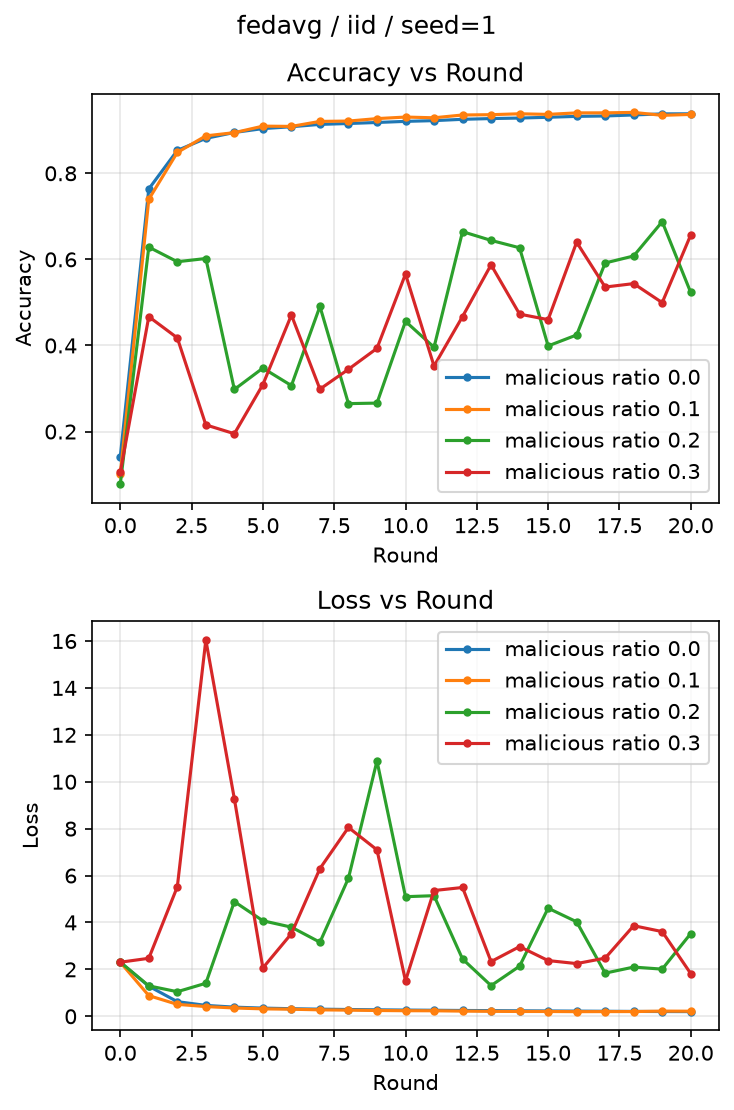
\includegraphics[width=\columnwidth]{result/fedavg_iid_seed1_by_ratio.png}
    \caption{FedAvg・IID・Seed 1 における malicious ratio 別の
    Round-Accuracy および Round-Loss の推移}
    \label{fig:fedavg_iid_seed1_by_ratio}
\end{figure}

\subsection{FedAvg（Non-IID環境）における悪性クライアント比率別の評価}

\subsubsection{実験条件}

FedAvgを用いたNon-IID環境において，悪性クライアント比率を変化させ，
悪性クライアント比率がモデルの性能に与える影響を比較する．
以下の条件はすべての実験で共通とした．

\begin{itemize}
    \item \textbf{Aggregation Method：} FedAvg
    \item \textbf{Data Split：} Non-IID
    \item \textbf{Attack：} Adaptive Attack
    \item \textbf{Number of Rounds：} 20
    \item \textbf{Seeds：} 1，2，3
\end{itemize}

比較対象とする悪性クライアント比率を以下に示す．

\begin{itemize}
    \item \textbf{Malicious Ratio：} 0.0，0.1，0.2，0.3
\end{itemize}

乱数の影響を考慮し，Seed値を1，2，3の3通り設定して実験を行った．
本文中の図には代表としてSeed 1の結果を示す．詳細な結果（全Seedの
推移）は付録に記載する．

\subsubsection{実験結果}

実験結果を図\ref{fig:fedavg_noniid_seed1_by_ratio}に示す．IID環境と
同様，Ratio 0.0，0.1ではAccuracyが概ね単調に0.87--0.94まで収束する．
Ratio 0.2，0.3ではIID環境と同様にAccuracyが0.1--0.7程度で振動し，
特にRatio 0.3ではLossがRound 6で11.2まで急上昇する．

定量的には，Round 5以降のRound間Accuracy変化量（絶対値平均）は
Ratio 0.0で0.0027，Ratio 0.1で0.0233，Ratio 0.2で0.1077，Ratio 0.3
で0.0818であり，Ratio 0.1の時点で既にRatio 0.0の約8.6倍の変動が
生じている．これはIID環境（Ratio 0.1の変化量0.0036）と比べて明確に
大きく，Non-IID環境の方が低いMalicious Ratioでも不安定化しやすい
ことを示唆する．最終AccuracyはRatio 0.0の$0.935\pm0.002$から
Ratio 0.1で$0.879\pm0.054$，Ratio 0.2で$0.675\pm0.062$，Ratio 0.3で
$0.665\pm0.045$まで低下し，IID環境（Ratio 0.1で$0.936\pm0.006$）より
先にSeed間ばらつきが顕在化する．この傾向は，Non-IID環境ではhonest
クライアント間の更新のばらつきが元々大きく，悪性クライアントの更新が
その中に紛れ込みやすいためと考えられ，\ref{sec:push_ratio_analysis}節のpush\_ratio分析の
結果とも整合する．

\begin{figure}[H]
    \centering
    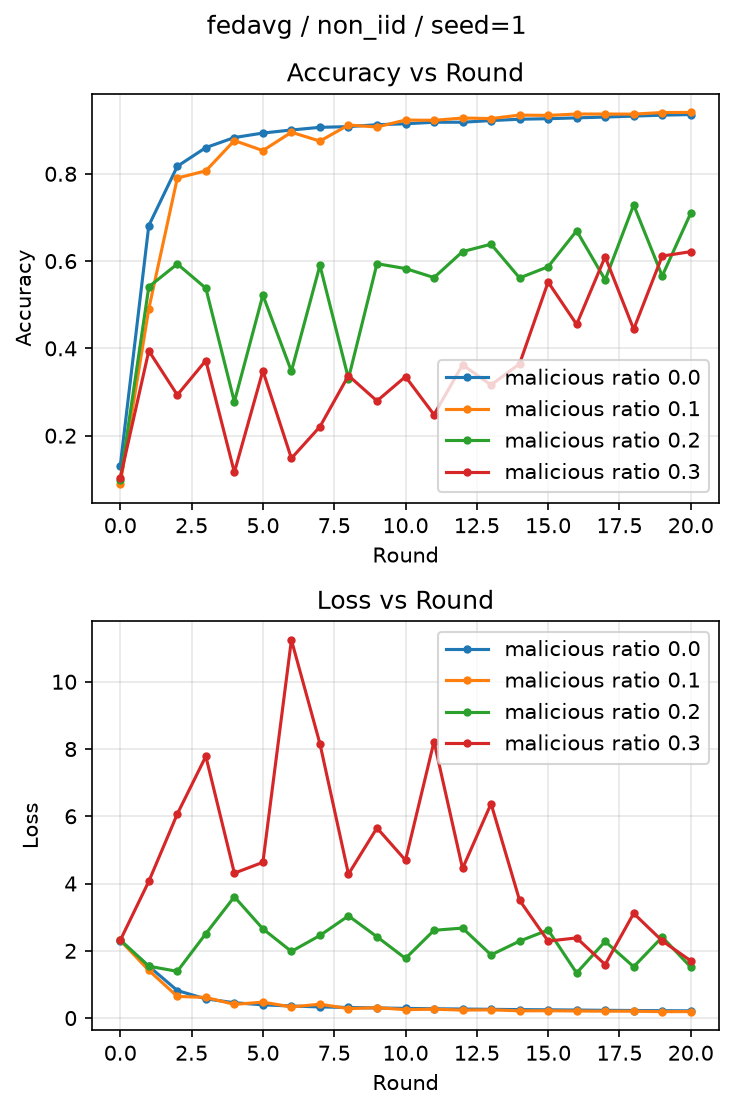
\includegraphics[width=\columnwidth]{result/fedavg_noniid_seed1_by_ratio.png}
    \caption{FedAvg・Non-IID・Seed 1 における malicious ratio 別の
    Round-Accuracy および Round-Loss の推移}
    \label{fig:fedavg_noniid_seed1_by_ratio}
\end{figure}

\subsection{Median（IID環境）における悪性クライアント比率別の評価}

\subsubsection{実験条件}

Medianを用いたIID環境において，悪性クライアント比率を変化させ，
悪性クライアント比率がモデルの性能に与える影響を比較する．
以下の条件はすべての実験で共通とした．

\begin{itemize}
    \item \textbf{Aggregation Method：} Median
    \item \textbf{Data Split：} IID
    \item \textbf{Attack：} Adaptive Attack
    \item \textbf{Number of Rounds：} 20
    \item \textbf{Seeds：} 1，2，3
\end{itemize}

比較対象とする悪性クライアント比率を以下に示す．

\begin{itemize}
    \item \textbf{Malicious Ratio：} 0.0，0.1，0.2，0.3
\end{itemize}

乱数の影響を考慮し，Seed値を1，2，3の3通り設定して実験を行った．
本文中の結果にはSeed 1の結果を採用する．詳細な結果（全Seedの推移）
は付録に記載する．

\subsubsection{実験結果}

実験結果を図\ref{fig:median_iid_seed1_by_ratio}に示す．全Ratio
（0.0--0.3）でAccuracyはRound 5までにほぼ収束し，以降は単調に
0.89--0.94程度で推移する．Lossも同様に単調減少し，FedAvgで見られた
ような振動は観測されない．

Ratioが大きいほど収束後のAccuracyはわずかに低下するが（Seed平均
$0.939\pm0.003$（Ratio 0.0）から$0.895\pm0.000$（Ratio 0.3）），
その差は0.05以下に留まる．Round 5以降のRound間Accuracy変化量
（絶対値平均）も全Ratioで0.001--0.003程度と小さく，Ratioによらず
ほぼ一定である．Seed間のばらつきも全Ratioで標準偏差0.003以下と
極めて小さく，MedianはIID環境において検証した範囲でAdaptive Model
Poisoning Attackに対して高い安定性を示した．

\begin{figure}[H]
    \centering
    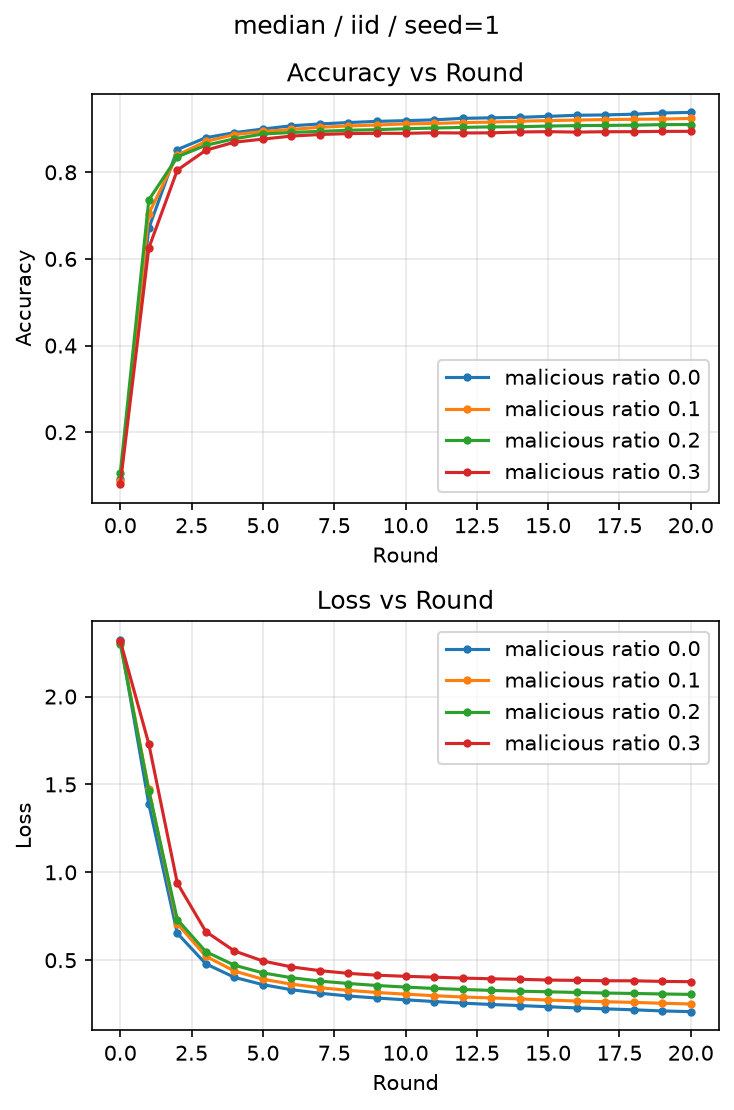
\includegraphics[width=\columnwidth]{result/median_iid_seed1_by_ratio.png}
    \caption{Median・IID・Seed 1 における malicious ratio 別の
    Round-Accuracy および Round-Loss の推移}
    \label{fig:median_iid_seed1_by_ratio}
\end{figure}

\subsection{Median（Non-IID環境）における悪性クライアント比率別の評価}

\subsubsection{実験条件}

Medianを用いたNon-IID環境において，悪性クライアント比率を変化させ，
悪性クライアント比率がモデルの性能に与える影響を比較する．
以下の条件はすべての実験で共通とした．

\begin{itemize}
    \item \textbf{Aggregation Method：} Median
    \item \textbf{Data Split：} Non-IID
    \item \textbf{Attack：} Adaptive Attack
    \item \textbf{Number of Rounds：} 20
    \item \textbf{Seeds：} 1，2，3
\end{itemize}

比較対象とする悪性クライアント比率を以下に示す．

\begin{itemize}
    \item \textbf{Malicious Ratio：} 0.0，0.1，0.2，0.3
\end{itemize}

乱数の影響を考慮し，Seed値を1，2，3の3通り設定して実験を行った．
本文中の結果にはSeed 1の結果を採用するが，Malicious Ratio 0.3の
Seed 1はRound 1でログが途切れているため，該当条件のみSeed 2，3を
含めた集計値を次項で併記する．詳細な結果（全Seedの推移）は付録に
記載する．

\subsubsection{実験結果}

実験結果を図\ref{fig:median_noniid_seed1_by_ratio}に示す．IID環境と
同様，全Ratioで振動のない滑らかな収束を示す．図中のRatio 0.3の系列
はSeed 1のログが途切れているためRound 0--1のみとなっているが，
Seed 2，3を含めた集計ではRatio 0.3の最終Accuracyは
$0.870\pm0.007$（$n=2$）であり，他のRatio（標準偏差0.001--0.002）
よりもやや大きいばらつきを示す．Round 5以降のRound間Accuracy変化量
もRatio 0.0--0.2では0.002--0.003程度で推移するのに対し，Ratio 0.3
では0.0075とやや増加しており，Non-IID環境かつ高Ratioでは学習後期の
安定性がわずかに低下する傾向がみられる．ただし，この変化幅はFedAvg
やKrumで見られる振動（後述）と比べると小さく，Medianは全体として
Non-IID環境でも比較的ロバストであるといえる．

\begin{figure}[H]
    \centering
    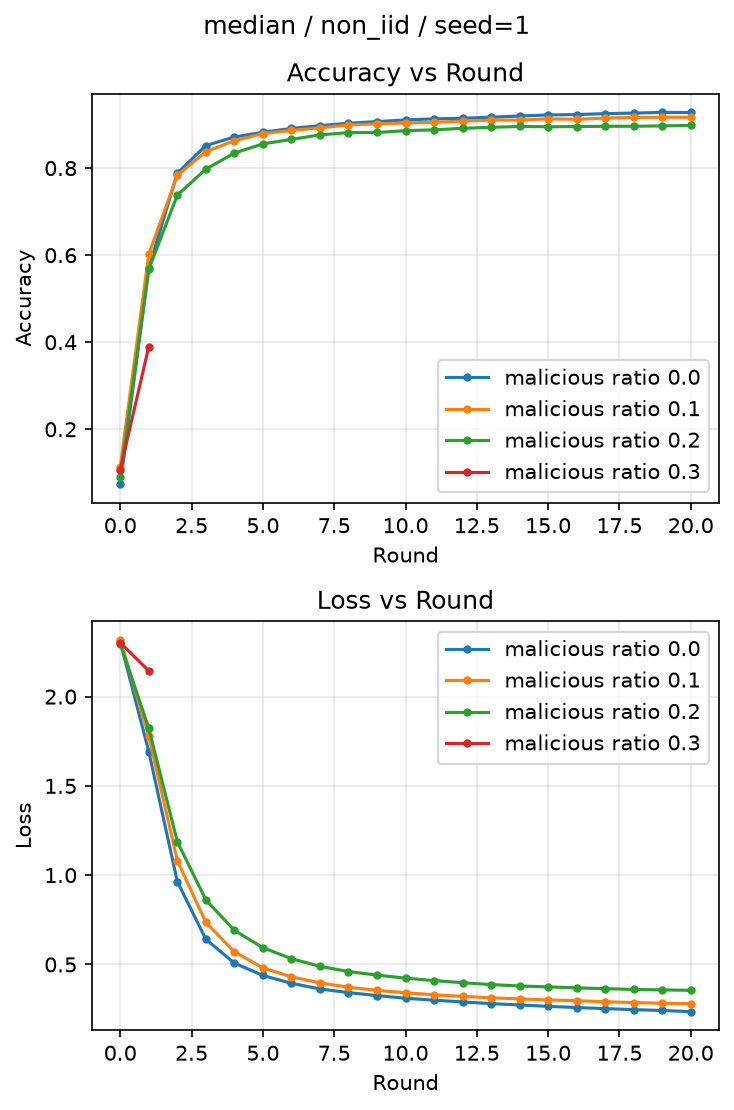
\includegraphics[width=\columnwidth]{result/median_noniid_seed1_by_ratio.png}
    \caption{Median・Non-IID・Seed 1 における malicious ratio 別の
    Round-Accuracy および Round-Loss の推移（malicious ratio 0.3 は
    Round 0--1 のみ）}
    \label{fig:median_noniid_seed1_by_ratio}
\end{figure}

\subsection{Trimmed Mean（IID環境）における悪性クライアント比率別の評価}

\subsubsection{実験条件}

Trimmed Meanを用いたIID環境において，悪性クライアント比率を変化させ，
悪性クライアント比率がモデルの性能に与える影響を比較する．
以下の条件はすべての実験で共通とした．

\begin{itemize}
    \item \textbf{Aggregation Method：} Trimmed Mean
    \item \textbf{Data Split：} IID
    \item \textbf{Attack：} Adaptive Attack
    \item \textbf{Number of Rounds：} 20
    \item \textbf{Seeds：} 1，2，3
\end{itemize}

比較対象とする悪性クライアント比率を以下に示す．

\begin{itemize}
    \item \textbf{Malicious Ratio：} 0.0，0.1，0.2，0.3
\end{itemize}

乱数の影響を考慮し，Seed値を1，2，3の3通り設定して実験を行った．
本文中の結果にはSeed 1の結果を採用する．詳細な結果（全Seedの推移）
は付録に記載する．

\subsubsection{実験結果}

実験結果を図\ref{fig:trimmed_mean_iid_seed1_by_ratio}に示す．Median
のIID環境と同様，全Ratioで振動のない滑らかな収束を示す．最終Accuracy
はRatio 0.0の$0.937\pm0.002$からRatio 0.3の$0.885\pm0.004$まで単調に
低下するが，Seed間の標準偏差はいずれも0.004以下と小さい．Round 5
以降のRound間Accuracy変化量も0.001--0.003程度でRatioによらず安定
しており，Trimmed MeanはIID環境において検証範囲内でMedianと同水準の
ロバスト性を示した．

\begin{figure}[H]
    \centering
    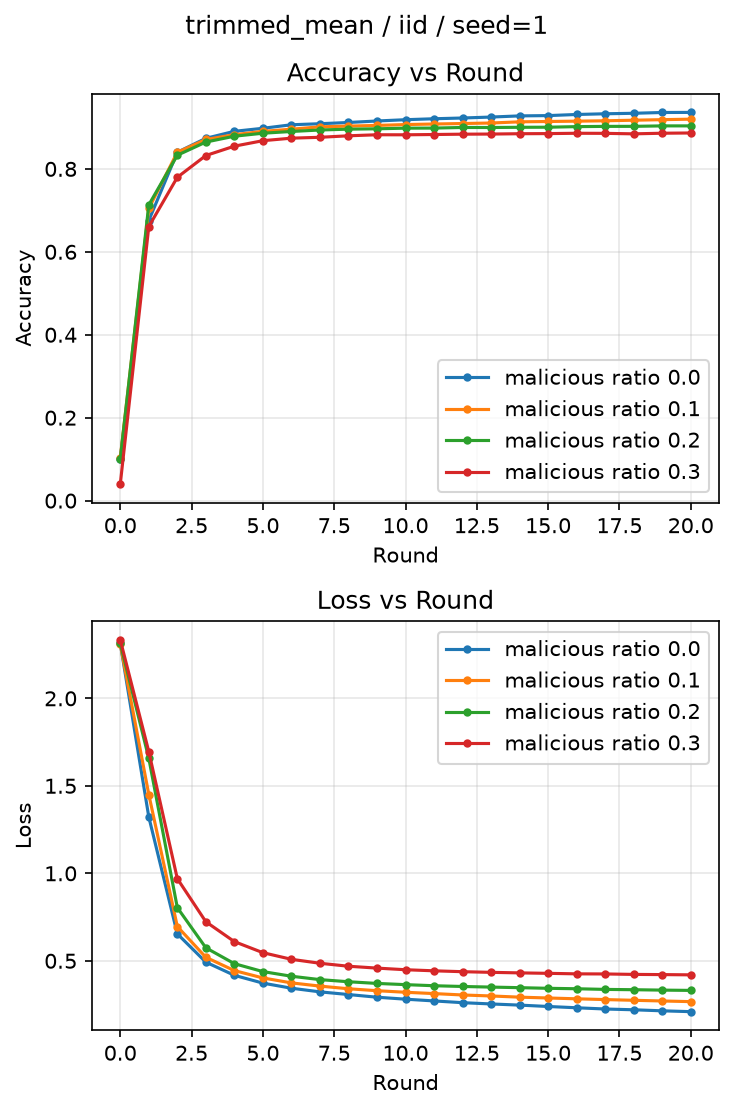
\includegraphics[width=\columnwidth]{result/trimmed_mean_iid_seed1_by_ratio.png}
    \caption{Trimmed Mean・IID・Seed 1 における malicious ratio 別の
    Round-Accuracy および Round-Loss の推移}
    \label{fig:trimmed_mean_iid_seed1_by_ratio}
\end{figure}

\subsection{Trimmed Mean（Non-IID環境）における悪性クライアント比率別の評価}

\subsubsection{実験条件}

Trimmed Meanを用いたNon-IID環境において，悪性クライアント比率を
変化させ，悪性クライアント比率がモデルの性能に与える影響を比較する．
以下の条件はすべての実験で共通とした．

\begin{itemize}
    \item \textbf{Aggregation Method：} Trimmed Mean
    \item \textbf{Data Split：} Non-IID
    \item \textbf{Attack：} Adaptive Attack
    \item \textbf{Number of Rounds：} 20
    \item \textbf{Seeds：} 1，2，3
\end{itemize}

比較対象とする悪性クライアント比率を以下に示す．

\begin{itemize}
    \item \textbf{Malicious Ratio：} 0.0，0.1，0.2，0.3
\end{itemize}

乱数の影響を考慮し，Seed値を1，2，3の3通り設定して実験を行った．
本節ではSeed 1のみの結果ではなく，Malicious Ratioごとに
Seed 1，2，3の平均値と標準偏差を算出し，平均線と標準偏差の帯を
重ねて比較する．詳細な結果（全Seedの推移）は付録に記載する．

\subsubsection{実験結果}

実験結果を図\ref{fig:trimmed_mean_noniid_seedmean_by_ratio}に示す．
Ratio 0.0--0.2はSeed間の標準偏差帯が細く，収束後は0.89--0.93程度で
安定する．一方Ratio 0.3のみ収束が明らかに遅く，Round 10付近まで
緩やかに上昇を続けるうえ，標準偏差帯も広い．

最終AccuracyはRatio 0.0の$0.930\pm0.001$からRatio 0.2の
$0.891\pm0.002$までは差が小さいが，Ratio 0.3では
$0.807\pm0.056$（Seed別内訳：0.742，0.837，0.841）まで悪化し，標準
偏差は他Ratioの20倍以上に拡大する．Round 5以降のRound間Accuracy
変化量もRatio 0.3では0.0081と，他Ratio（0.0026--0.0030）の約3倍に
増加している．以上より，Trimmed MeanはNon-IID環境かつ悪性クライアント
比率が高い条件（Ratio 0.3）でのみ，Seedに依存した不安定な挙動を示す
ことが確認された．これは，Non-IID環境では座標ごとの分布形状も
クライアントによって偏るため，Trimmed Meanのトリム幅を上回る割合の
悪性クライアントが存在すると，除外しきれない悪性値が座標の平均に
混入しやすくなるためと考えられる．

\begin{figure}[H]
    \centering
    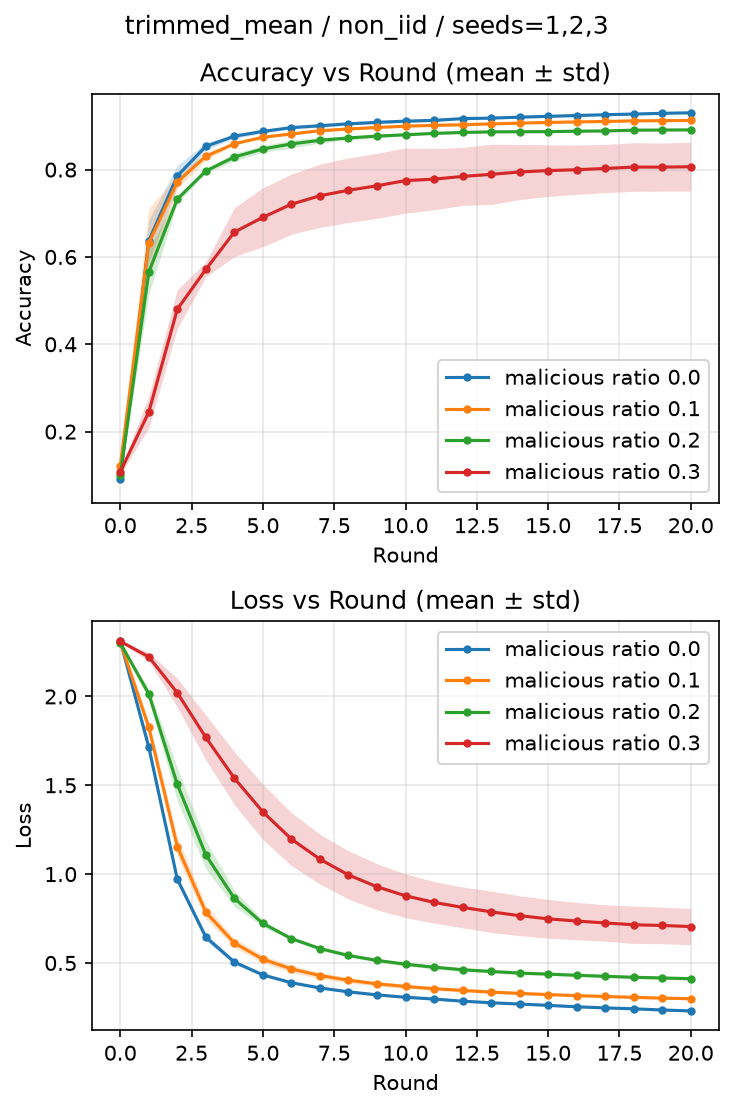
\includegraphics[width=\columnwidth]{result/trimmed_mean_noniid_seedmean_by_ratio.png}
    \caption{Trimmed Mean・Non-IID における malicious ratio 別の
    Round-Accuracy および Round-Loss の推移（Seed 1, 2, 3 の平均 $\pm$
    標準偏差）}
    \label{fig:trimmed_mean_noniid_seedmean_by_ratio}
\end{figure}

\subsection{Krum（IID環境）における悪性クライアント比率別の評価}

\subsubsection{実験条件}

Krumを用いたIID環境において，悪性クライアント比率を変化させ，
悪性クライアント比率がモデルの性能に与える影響を比較する．
以下の条件はすべての実験で共通とした．

\begin{itemize}
    \item \textbf{Aggregation Method：} Krum
    \item \textbf{Data Split：} IID
    \item \textbf{Attack：} Adaptive Attack
    \item \textbf{Number of Rounds：} 20
    \item \textbf{Seeds：} 1，2，3
\end{itemize}

比較対象とする悪性クライアント比率を以下に示す．

\begin{itemize}
    \item \textbf{Malicious Ratio：} 0.0，0.1，0.2，0.3
\end{itemize}

乱数の影響を考慮し，Seed値を1，2，3の3通り設定して実験を行った．
Krumは複数クライアントの更新を平均せず1クライアントの更新のみを
採用する集約手法であるため，本節ではSeed 1のみの結果ではなく，
Malicious Ratioごとに Seed 1，2，3（一部Roundでログが途切れたSeedを
除く）の平均値と標準偏差を算出し，平均線と標準偏差の帯を重ねて比較
する．詳細な結果（全Seedの推移）は付録に記載する．

\subsubsection{実験結果}

実験結果を図\ref{fig:krum_iid_seedmean_by_ratio}に示す．Malicious
Ratio 0.0でも収束後のAccuracyは0.87--0.93程度で細かく上下しており，
Round 5以降のRound間Accuracy変化量（絶対値平均）は0.0103と，Median・
Trimmed MeanのRatio 0.0（いずれも0.0026）の約4倍に達する．これは
Krumが毎ラウンド1クライアントのみを選択する構造上，選ばれるクライアント
がラウンドごとに入れ替わることに起因すると考えられる（要因の詳細は
\ref{sec:krum_bulyan_spread_analysis}節で分析する）．

Malicious Ratio 0.2，0.3では，Accuracyが学習中盤で一度ピークに達した
後，終盤にかけて低下するという他手法には見られない挙動が確認された．
Ratio 0.2ではRound 8で0.844まで上昇した後，Round 20には0.761まで
低下し（$-0.083$），Ratio 0.3ではRound 7で0.728まで上昇した後，
Round 20には0.429まで低下する（$-0.299$）．最終Accuracy
（Seed平均$\pm$標準偏差）はRatio 0.0の$0.903\pm0.009$から
Ratio 0.2で$0.761\pm0.049$，Ratio 0.3で$0.429\pm0.041$（$n=2$，
一部Seedのログ欠損のため）まで悪化する．Round 5以降のRound間
Accuracy変化量もRatio 0.3で0.0283とRatio 0.0の約2.7倍に拡大して
いる．この「中盤でピークに達した後に劣化する」挙動は，Adaptive
Model Poisoning Attackが学習の進行に伴い悪性更新をKrumに選択され
やすい形へ最適化し続けることで，防御が徐々に破綻していく過程を
反映していると考えられる．

\begin{figure}[H]
    \centering
    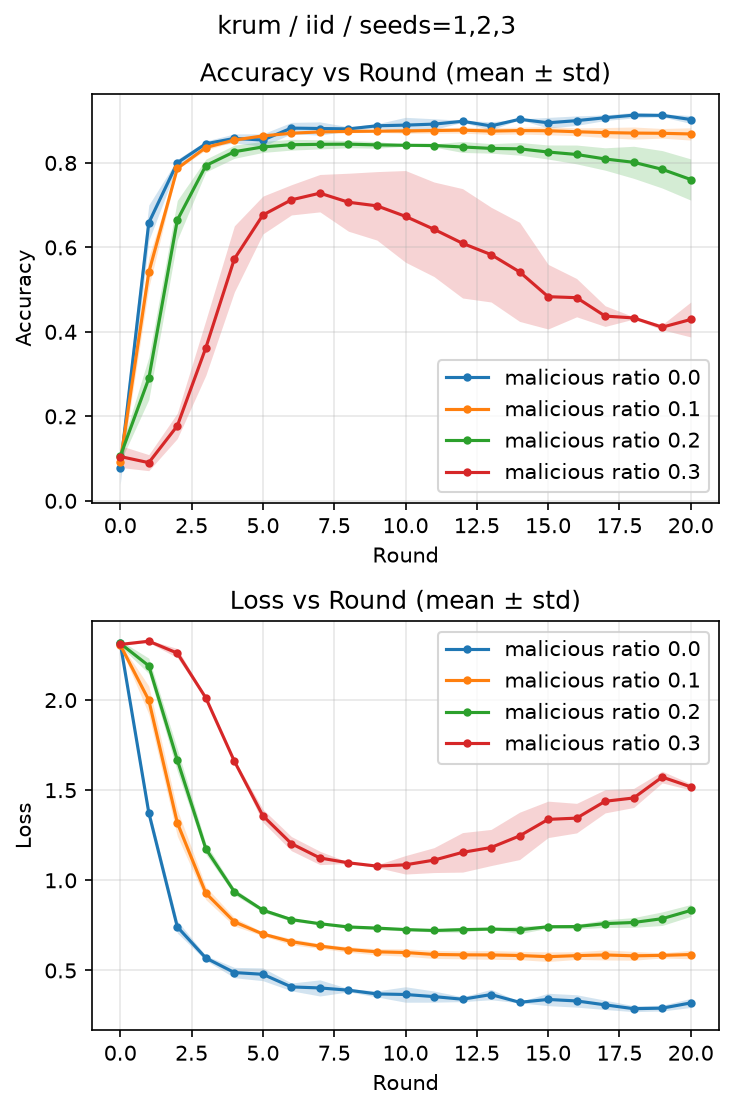
\includegraphics[width=\columnwidth]{result/krum_iid_seedmean_by_ratio.png}
    \caption{Krum・IID における malicious ratio 別の
    Round-Accuracy および Round-Loss の推移（Seed 平均 $\pm$
    標準偏差）}
    \label{fig:krum_iid_seedmean_by_ratio}
\end{figure}

\subsection{Krum（Non-IID環境）における悪性クライアント比率別の評価}

\subsubsection{実験条件}

Krumを用いたNon-IID環境において，悪性クライアント比率を変化させ，
悪性クライアント比率がモデルの性能に与える影響を比較する．
以下の条件はすべての実験で共通とした．

\begin{itemize}
    \item \textbf{Aggregation Method：} Krum
    \item \textbf{Data Split：} Non-IID
    \item \textbf{Attack：} Adaptive Attack
    \item \textbf{Number of Rounds：} 20
    \item \textbf{Seeds：} 1，2，3
\end{itemize}

比較対象とする悪性クライアント比率を以下に示す．

\begin{itemize}
    \item \textbf{Malicious Ratio：} 0.0，0.1，0.2，0.3
\end{itemize}

乱数の影響を考慮し，Seed値を1，2，3の3通り設定して実験を行った．
IID環境の場合と同様，本節でもMalicious RatioごとにSeed 1，2，3
（一部Roundでログが途切れたSeedを除く）の平均値と標準偏差を算出し，
平均線と標準偏差の帯を重ねて比較する．詳細な結果（全Seedの推移）は
付録に記載する．

\subsubsection{実験結果}

実験結果を図\ref{fig:krum_noniid_seedmean_by_ratio}に示す．Malicious
Ratio 0.0における収束後のRound間Accuracy変化量（絶対値平均，
Round 5以降）は0.0678であり，同条件のIID環境（0.0103）の約6.6倍に
達する．IID環境ではbenign\_spread（honestクライアント間の分散）が
Round 5以降ほぼ横ばいで推移するのに対し，Non-IID環境ではクライアント
ごとのローカルデータ分布が偏っているため，Krumが選択する少数の
クライアントがラウンドごとに入れ替わるたびにモデル品質が大きく変動
することが要因と考えられる（\ref{sec:krum_bulyan_spread_analysis}節で定量的に検証する）．

Malicious Ratio 0.2では，IID環境と同様に学習中盤（Round 11）で
0.748まで上昇した後，終盤（Round 20）には0.645まで低下する
（$-0.103$）．Ratio 0.3では，Accuracyが全期間を通じて0.1--0.2程度に
留まり，最終Accuracyは$0.199\pm0.109$（$n=2$，Seed別内訳：0.276，
0.122）と学習がほぼ成立していない．Lossも他Ratioが1.0前後に収束する
のに対し，Ratio 0.3ではRound 10以降も3.3--3.7程度の高い値で推移し，
標準偏差帯も非常に広い．以上より，KrumはNon-IID環境において
Malicious Ratio 0.0の時点から構造的に不安定であり，Ratio 0.3では
Adaptive Model Poisoning Attackに対してほぼ防御が機能しないことが
確認された．

\begin{figure}[H]
    \centering
    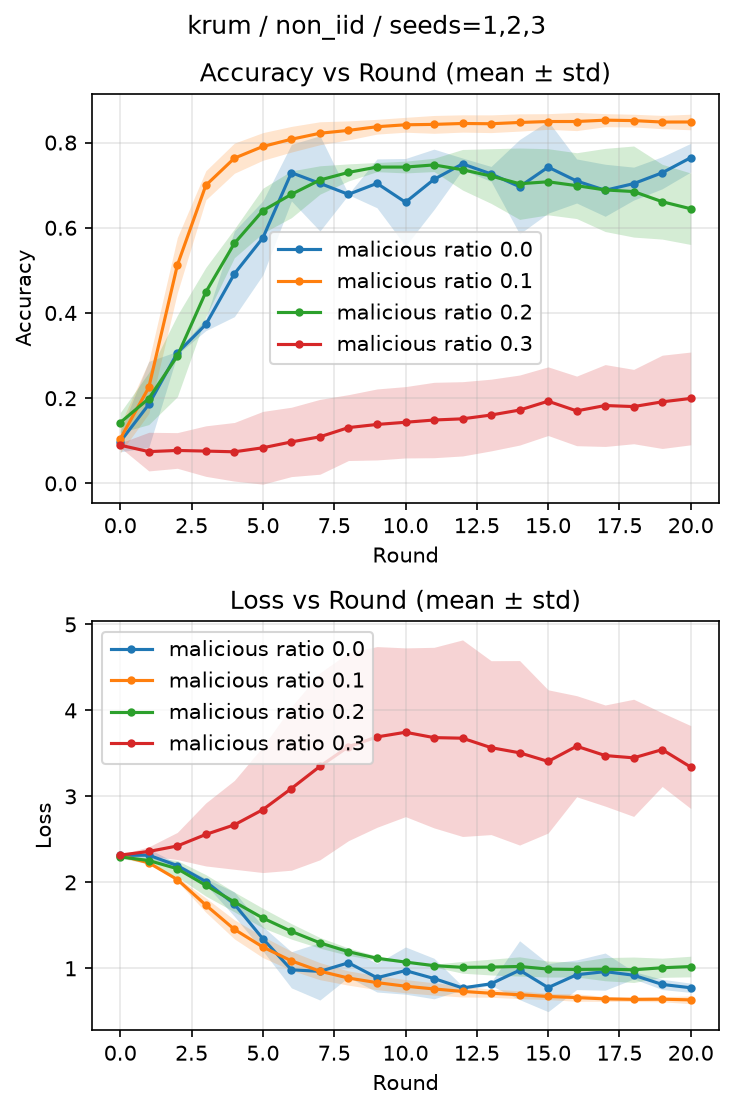
\includegraphics[width=\columnwidth]{result/krum_noniid_seedmean_by_ratio.png}
    \caption{Krum・Non-IID における malicious ratio 別の
    Round-Accuracy および Round-Loss の推移（Seed 平均 $\pm$
    標準偏差）}
    \label{fig:krum_noniid_seedmean_by_ratio}
\end{figure}

\subsection{Bulyan（IID環境）における悪性クライアント比率別の評価}

\subsubsection{実験条件}

Bulyanを用いたIID環境において，悪性クライアント比率を変化させ，
悪性クライアント比率がモデルの性能に与える影響を比較する．
以下の条件はすべての実験で共通とした．

\begin{itemize}
    \item \textbf{Aggregation Method：} Bulyan
    \item \textbf{Data Split：} IID
    \item \textbf{Attack：} Adaptive Attack
    \item \textbf{Number of Rounds：} 20
    \item \textbf{Seeds：} 1，2，3
\end{itemize}

比較対象とする悪性クライアント比率を以下に示す．

\begin{itemize}
    \item \textbf{Malicious Ratio：} 0.0，0.1，0.2
\end{itemize}

乱数の影響を考慮し，Seed値を1，2，3の3通り設定して実験を行った．
Malicious Ratio 0.3（$f=30$）はBulyanのロバスト性条件
$n \geq 4f+3$（$100 < 123$）を満たさず，Round 0以降のログが存在しない
ため，本節の比較対象から除外する．他章との表記統一のため，Malicious
RatioごとにSeed 1，2，3の平均値と標準偏差を算出し，平均線と標準偏差
の帯を重ねて比較する．詳細な結果（全Seedの推移）は付録に記載する．

\subsubsection{実験結果}

実験結果を図\ref{fig:bulyan_iid_seedmean_by_ratio}に示す．全Ratio
（0.0--0.2）でAccuracyは振動なく単調に収束し，KrumのIID環境で見られた
ような中盤ピーク後の低下も見られない．最終AccuracyはRatio 0.0の
$0.939\pm0.002$（$n=2$）からRatio 0.2の$0.901\pm0.001$までわずかに
低下するのみである．Round 5以降のRound間Accuracy変化量も
0.0017--0.0025とRatioによらず小さく，同一Ratio帯のKrum
（0.0076--0.0103）と比べて明確に安定している．Bulyanは複数の候補
クライアントを集約したうえで外れ値を除去する多段構成であるため，
Krumのように単一の選択結果に強く依存せず，IID環境では悪性クライアント
比率の増加に対しても安定した挙動を維持することが確認された．

\begin{figure}[H]
    \centering
    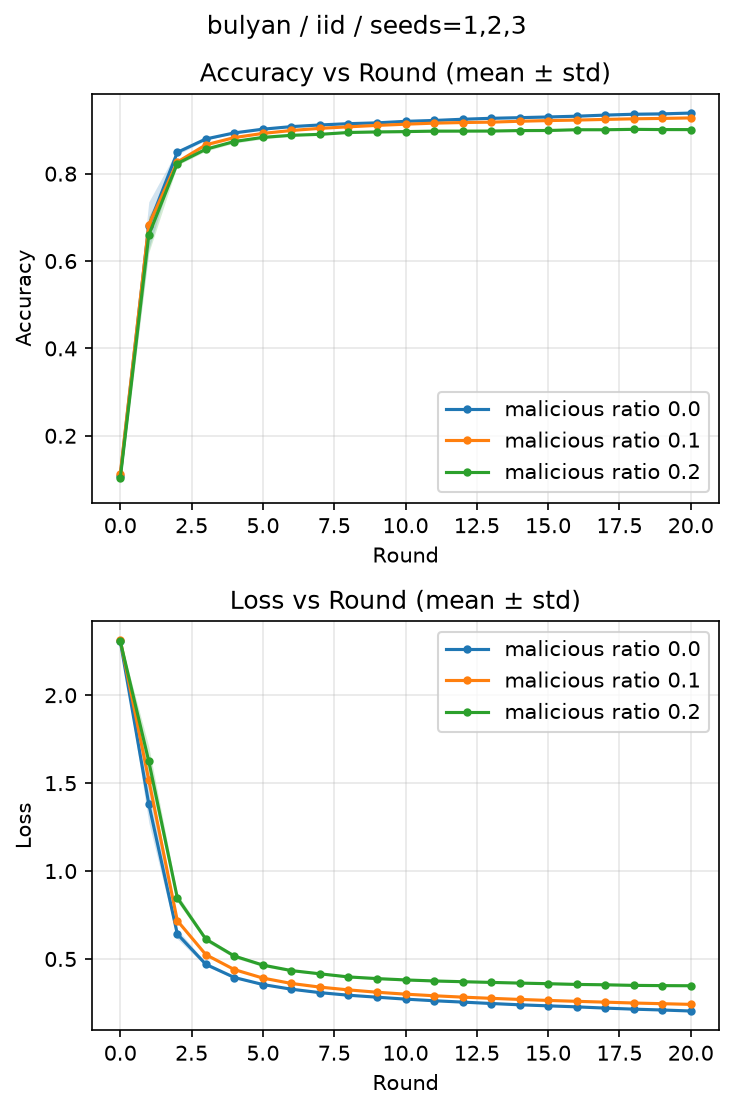
\includegraphics[width=\columnwidth]{result/bulyan_iid_seedmean_by_ratio.png}
    \caption{Bulyan・IID における malicious ratio 別の
    Round-Accuracy および Round-Loss の推移（Seed 平均 $\pm$
    標準偏差，malicious ratio 0.3 はロバスト性条件を満たさないため
    対象外）}
    \label{fig:bulyan_iid_seedmean_by_ratio}
\end{figure}

\subsection{Bulyan（Non-IID環境）における悪性クライアント比率別の評価}

\subsubsection{実験条件}

Bulyanを用いたNon-IID環境において，悪性クライアント比率を変化させ，
悪性クライアント比率がモデルの性能に与える影響を比較する．
以下の条件はすべての実験で共通とした．

\begin{itemize}
    \item \textbf{Aggregation Method：} Bulyan
    \item \textbf{Data Split：} Non-IID
    \item \textbf{Attack：} Adaptive Attack
    \item \textbf{Number of Rounds：} 20
    \item \textbf{Seeds：} 1，2，3
\end{itemize}

比較対象とする悪性クライアント比率を以下に示す．

\begin{itemize}
    \item \textbf{Malicious Ratio：} 0.0，0.1，0.2
\end{itemize}

乱数の影響を考慮し，Seed値を1，2，3の3通り設定して実験を行った．
IID環境の場合と同様，Malicious Ratio 0.3（$f=30$）はBulyanの
ロバスト性条件 $n \geq 4f+3$（$100 < 123$）を満たさず，Round 0以降の
ログが存在しないため，本節の比較対象から除外する．Malicious Ratio
ごとにSeed 1，2，3の平均値と標準偏差を算出し，平均線と標準偏差の帯を
重ねて比較する．詳細な結果（全Seedの推移）は付録に記載する．

\subsubsection{実験結果}

実験結果を図\ref{fig:bulyan_noniid_seedmean_by_ratio}に示す．IID環境
と同様，全Ratioで振動のない滑らかな収束を示す．最終Accuracyは
Ratio 0.0の$0.930\pm0.003$からRatio 0.1の$0.917\pm0.002$までは差が
小さいが，Ratio 0.2では$0.833\pm0.026$まで低下し，収束もやや遅く
なる（Accuracyが0.8台に達するのがRound 10以降）．それでもRound 5
以降のRound間Accuracy変化量はRatio 0.2で0.0064にとどまり，同一Ratio
帯のKrum Non-IID（0.0171）やFedAvg Non-IID（0.1077）と比べて一桁
小さい．以上より，Bulyanは実行可能なRatio範囲（0.0--0.2）において
Non-IID環境でも他手法より高い安定性を維持するが，Ratio 0.2で標準
偏差が拡大し始めている点は，ロバスト性条件の上限（Ratio 0.25で
$n<4f+3$）に近づくにつれて余裕が減少していることを示唆している．

\begin{figure}[H]
    \centering
    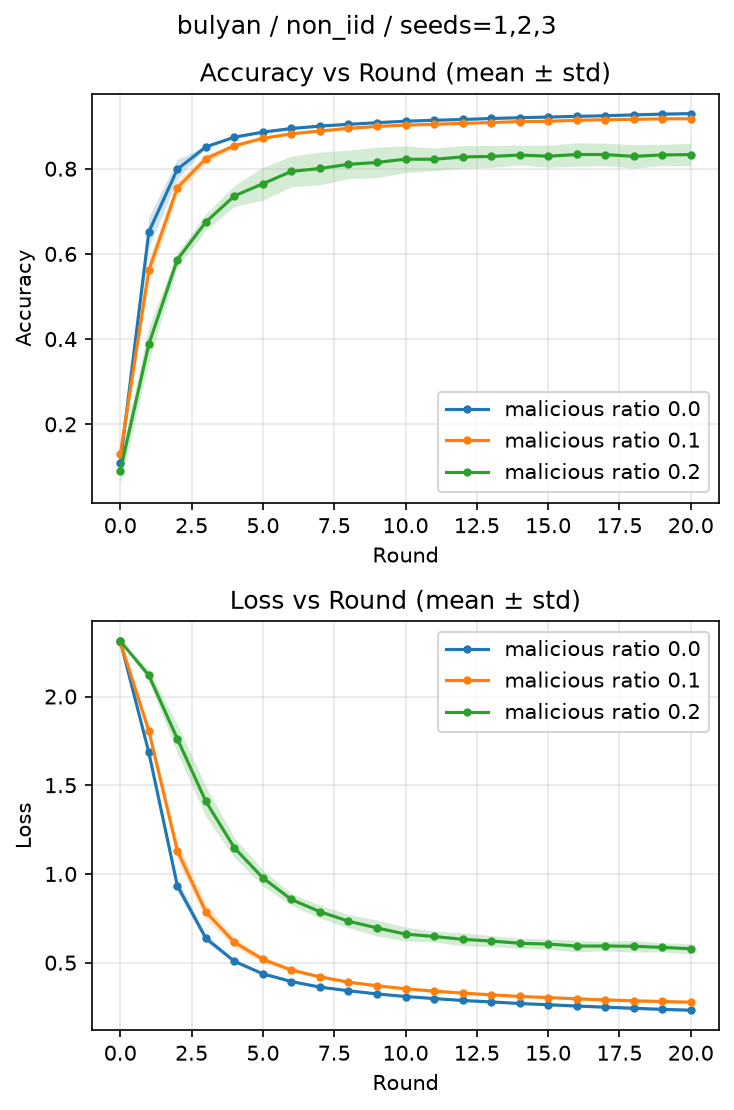
\includegraphics[width=\columnwidth]{result/bulyan_noniid_seedmean_by_ratio.png}
    \caption{Bulyan・Non-IID における malicious ratio 別の
    Round-Accuracy および Round-Loss の推移（Seed 平均 $\pm$
    標準偏差，malicious ratio 0.3 はロバスト性条件を満たさないため
    対象外）}
    \label{fig:bulyan_noniid_seedmean_by_ratio}
\end{figure}

\section{追加実験:Robust Aggregation の失敗モードに関する定量分析計画書}

\subsection{目的}

本文書は，\texttt{sotsuron\_plan.tex}で報告した実験結果（Adaptive Model Poisoning Attackに対する各Robust Aggregation手法の耐性評価）のうち，特に挙動の異なる4つの現象について，その要因を定量的に分析するための計画をまとめる。

Fang ら\cite{fang2020local}のAdaptive Model Poisoning Attackは，Robust Aggregation手法が防御として不十分であることを攻撃成功率の観点から示したが，「なぜ・どの条件で防御が破綻するのか」というメカニズムには踏み込んでいない。本研究では，既存実験で観測された以下の現象を手がかりに，この問いに定量的な説明を与えることを目指す。

\subsection{観測された現象}

\begin{itemize}
  \item Krum / Bulyanは，Malicious Ratio 0.0（悪性クライアント不在）の場合でもラウンドごとの精度変動が大きい。
  \item FedAvgは，Malicious Ratio 0.2以上でAccuracy・Lossがラウンドごとに大きく振動する。
  \item Trimmed MeanをNon-IID環境で用いた場合，Malicious Ratio 0.3のときのみSeed間で最終Accuracyが0.74--0.84と大きくばらつく（他のMalicious Ratioでは Seed間差は0.01未満）。
  \item Bulyanはロバスト性条件 $n \geq 4f+3$ を満たさないMalicious Ratio 0.3（$100 < 123$）において，原理的に動作しない。
\end{itemize}

4点目は集約手法の数式上の制約から自明に説明できるため考察のみで扱い，1--3点目について新たな定量指標を導入して分析する。

\subsection{提案する分析指標}

\subsubsection{honestクラスタの分散（benign spread）}

各ラウンドにおいて，honestなクライアント更新の重心 $\bar{v}_{\text{benign}}$ からの平均距離を次式で定義する。

\begin{equation}
\text{spread} = \frac{1}{|B|}\sum_{i \in B} \|v_i - \bar{v}_{\text{benign}}\|_2
\end{equation}

ここで $B$ はhonestクライアントの添字集合，$v_i$ はクライアント $i$ の更新ベクトルである。IID環境よりNon-IID環境の方がこの値が大きくなることが予想される。

\subsubsection{maliciousの押し出し距離と push ratio}

攻撃適用後のmalicious更新ベクトルについても同様に，honest重心からの平均距離を求める。

\begin{equation}
\text{push} = \frac{1}{|M|}\sum_{i \in M} \|v_i - \bar{v}_{\text{benign}}\|_2
\end{equation}

両者の比

\begin{equation}
\text{push\_ratio} = \frac{\text{push}}{\text{spread}}
\end{equation}

を定義する。push\_ratioが小さいほど，malicious更新はhonestクラスタの分布に紛れやすく，検出・排除されにくいと解釈できる。「Non-IID環境ではhonest同士の分散が元々大きいためpush\_ratioが小さくなり，攻撃が識別されにくい」という仮説をこの指標で検証する。

\subsubsection{Krum選択結果}

KrumおよびBulyanの内部選択において，選ばれたクライアントがmaliciousかhonestかを2値 \texttt{krum\_selected\_malicious} として各ラウンド記録する。Malicious Ratio 0.0でも生じる精度変動が，honestクライアント間のどのような差異に起因するかをこの記録とspreadの推移から考察する。

\subsubsection{Trimmed Meanにおける生存率（今後の課題）}

Trimmed Meanは座標ごとに上位・下位 $\beta$ 個の値を除外してから平均を取るため，malicious更新が座標ごとに除外対象となるか否かで攻撃の効き方が変わる。座標ごとの順位を用いて，malicious更新が除外されずに生き残った座標の割合 \texttt{frac\_dims\_survived} を定義する。この指標は次元数が大きく計算コストが増えるため，まずは3.1--3.3節の指標を優先し，実装余力があれば追加する。

\subsection{実装方針}

上記指標は，\texttt{pytorchexample/robust\_strategy.py} の \texttt{aggregate\_train} 内，Adaptive Model Poisoning Attack適用後・集約前の時点で計算する。この時点で全クライアントの更新ベクトル \texttt{updates}，malicious添字 \texttt{malicious\_pos}，集約前のグローバルモデル \texttt{self.\_last\_global\_vector} がすでにメモリ上に存在するため，モデル全体のベクトルを新たに保存する必要はなく，ラウンドごとの要約統計量のみをCSVへ追記すればよい。

\subsection{実験対象条件}

新指標は既存ログ（\texttt{result/}, \texttt{logs/}）には含まれないため，再実験が必要である。全条件×Ratio細分化×Seed数増加を単純に掛け合わせると実行数が膨大になるため（後述の見積りで350〜400回，計算時間にして半日以上），\textbf{探索(Phase 1)}と\textbf{検証(Phase 2)}の2段階に分けて依存関係を切ることで，網羅性を保ちながら実行数を抑える。

\subsubsection{Phase 1：ベースグリッド＋Ratio細分化（探索）}

まずSeed数は3のまま，全手法・全条件を対象にRatio方向の解像度を上げて実行する。目的は「どの手法・どのデータ分布・どのRatio付近で不安定になるか」を広く安く特定することであり，この段階ではSeed間分布の精緻な推定は求めない。

\begin{itemize}
  \item 集約手法：FedAvg，Median，Trimmed Mean，Krum，Bulyanの5手法全て
  \item データ分布：IID・Non-IID
  \item Malicious Ratio：基本は0.0，0.1，0.2，0.3。加えて
    \begin{itemize}
      \item Trimmed Mean（Non-IID）：0.225，0.25，0.275を追加
      \item Krum・Bulyan：0.05刻みで0.0から実行可能上限（Bulyanは $n \geq 4f+3$ を満たす範囲）まで追加
      \item FedAvg：0.125，0.15，0.175を追加
    \end{itemize}
  \item Seed：3（全条件共通，据え置き）
\end{itemize}

概算実行数はFedAvg 42，Median 24，Trimmed Mean 33，Krum 42，Bulyan 30の計約171回（1回平均2分として約5.7時間）。

\subsubsection{Phase 2：Seed数増加（検証）}

Phase 1の結果，Seed間で最終Accuracyのばらつきが大きい（既存結果のTrimmed Mean Non-IID Ratio 0.3のような）ことが確認されたRatio点\textbf{のみ}を対象に，Seedを3から10へ増やして追加実行する（7 Seed分を追加）。全Ratio×全手法に一律でSeedを増やすことはしない。

現時点でSeed間ばらつきが疑われるのはKrum・Bulyan（元々Ratio 0.0でも変動が大きい）とTrimmed Mean（Non-IID，Ratio 0.2--0.3付近）だが，最終的な対象点はPhase 1の結果を見てから確定する。仮にKrum・Bulyanの全Ratio×IID/Non-IIDとTrimmed Mean Non-IIDの数点が対象になった場合，概算で追加70回程度（約2.3時間）。

Phase 1と2を合わせても総実行数は約240回・半日弱に収まり，全条件に10 Seed×細分化Ratioを単純に掛け合わせる場合（350〜400回）よりも大幅に抑えられる。

\subsection{Phase 1 実験結果}
\label{sec:phase1_results}

\subsubsection{実行結果の概要}

5.1節の設計に従い，5手法×IID/Non-IID×細分化Ratio×Seed 3の計171回を実行した（FedAvg 42，Median 24，Trimmed Mean 33，Krum 42，Bulyan 30）。実行中に起動直後のログストリーム接続失敗により8件が一時的に中断したが，いずれも再実行により正常終了しており，最終的な集計対象（\texttt{experiments\_phase1/\_logs/summary.csv}，171行）に欠損はない。BulyanはMalicious Ratio 0.25以降，ロバスト性条件 $n \geq 4f+3$（$n=100$）を満たさなくなるため計画通り実行対象から除外し，実行上限はRatio 0.2までとなった。

\subsubsection{Malicious Ratio に対する Accuracy の全体傾向}

図\ref{fig:phase1_accuracy_overview}に，手法・データ分布ごとの最終Accuracy（Seed平均±標準偏差）をRatio別に示す。Median・Trimmed Meanは検証した全Ratio（IID/Non-IIDとも0.3まで）でAccuracy 0.8以上を維持し，Bulyanも実行上限のRatio 0.2までほぼ単調に高い精度を保った。一方，KrumはRatioの増加とともに急激に劣化し，Ratio 0.3ではIID 0.420（範囲0.367--0.473），Non-IID 0.250（範囲0.174--0.382）まで低下する。FedAvgはRatio 0.125付近から精度が崩れ始め，Ratio 0.3ではIID 0.525，Non-IID 0.698まで低下するとともに，Seed間の誤差棒（後述の標準偏差）が他手法より一貫して大きい。

\begin{figure}[H]
    \centering
    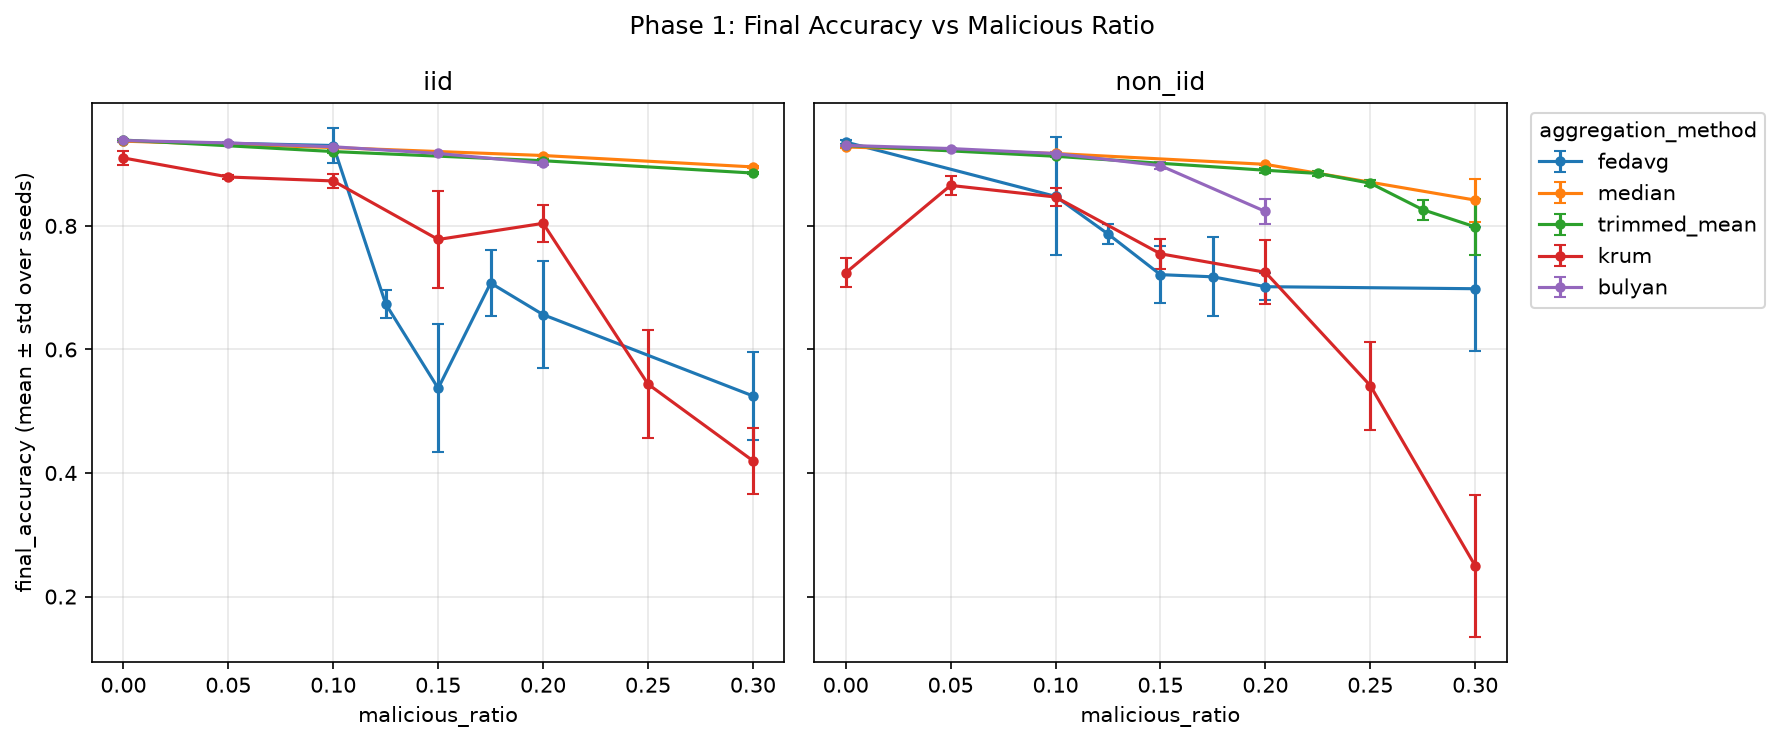
\includegraphics[width=\columnwidth]{experiments_phase1/analysis/accuracy_vs_ratio_overview.png}
    \caption{Phase 1：手法別・データ分布別のMalicious Ratio に対する最終Accuracy（Seed平均±標準偏差）}
    \label{fig:phase1_accuracy_overview}
\end{figure}

\subsubsection{Seed間ばらつきの特定（Phase 2候補点）}

条件（手法×データ分布×Ratio）ごとにSeed間の最終Accuracyの標準偏差を集計したところ（\texttt{seed\_variance.csv}），計画書2節の基準（他Ratioでは差0.01未満）を明確に上回るしきい値0.02以上の条件が57条件中23件見つかった。内訳はFedAvg 11件（IID 6，Non-IID 5），Krum 9件（IID 4，Non-IID 5），Trimmed Mean・Median・Bulyanが各1件（いずれもNon-IID）である。上位10件を表\ref{tab:phase1_seed_variance}に示す。

\begin{table}[H]
\centering
\caption{Seed間標準偏差が大きい上位10条件（acc\_std降順）}
\label{tab:phase1_seed_variance}
\footnotesize
\begin{tabular}{llccc}
\hline
手法 & 分布 & Ratio & acc\_mean & acc\_std \\
\hline
Krum & Non-IID & 0.30 & 0.250 & 0.1149 \\
FedAvg & IID & 0.15 & 0.537 & 0.1036 \\
FedAvg & Non-IID & 0.30 & 0.698 & 0.1001 \\
FedAvg & Non-IID & 0.10 & 0.848 & 0.0957 \\
Krum & IID & 0.25 & 0.544 & 0.0870 \\
FedAvg & IID & 0.20 & 0.656 & 0.0865 \\
Krum & IID & 0.15 & 0.778 & 0.0792 \\
FedAvg & IID & 0.30 & 0.525 & 0.0713 \\
Krum & Non-IID & 0.25 & 0.541 & 0.0711 \\
FedAvg & Non-IID & 0.175 & 0.718 & 0.0640 \\
\hline
\end{tabular}
\end{table}

計画段階で想定していたTrimmed Mean（Non-IID，Ratio 0.3，acc\_std=0.0456）は候補として残るものの，実際にはKrumとFedAvgがばらつきの主要因であることが分かった。特にKrum Non-IID Ratio 0.3は最終Accuracyが0.174--0.382とSeedによって攻撃の成否がほぼ反転しており，Phase 2でのSeed数増加（3→10）による検証が最も必要な条件といえる。

\subsubsection{push\_ratioによるIID/Non-IID間の紛れやすさの検証}
\label{sec:push_ratio_analysis}

Malicious Ratio $>0$ の全ラウンド・全Seedについて，手法・データ分布別にpush\_ratio（式(3)）の平均を集計した（図\ref{fig:phase1_push_ratio}）。Krum（IID 1.222 → Non-IID 0.853）およびBulyan（IID 1.090 → Non-IID 0.760）は，Non-IID環境で明確にpush\_ratioが低下しており，「Non-IID環境ではhonestクラスタの分散が元々大きいため攻撃が紛れやすい」という仮説と整合する。FedAvgも同様の傾向（IID 17.7 → Non-IID 13.4）を示すが，Median（10.25 → 10.54）とTrimmed Mean（10.20 → 10.28）ではIID/Non-IID間でほとんど差が見られなかった。これは，Median・Trimmed Meanが座標ごとの順位に基づく処理であり，クライアント間の全体的な距離構造（honestクラスタの形状）に依存しないためと考えられる。

また，Krum・Bulyanのpush\_ratioは1に近い値（1.0--1.2程度）である一方，FedAvg・Median・Trimmed Meanでは10--18程度と一桁大きい。前者は距離に基づく選抜（Krum選択・Bulyanの候補選定）を介するため，Fangらの最適化型攻撃はhonestクラスタから見て「選ばれる範囲でぎりぎり最大」となるようpush幅を調整しており，結果としてpush\_ratioがhonest同士の分散とほぼ同水準に収束する。一方，選抜を経ないFedAvgや，座標単位の順位処理のみのMedian・Trimmed Meanでは，攻撃者は選抜による排除を恐れずに大きくpushでき，push\_ratioが著しく大きくなる。これは次項のFedAvgの振動増大の一因と考えられる。

\begin{figure}[H]
    \centering
    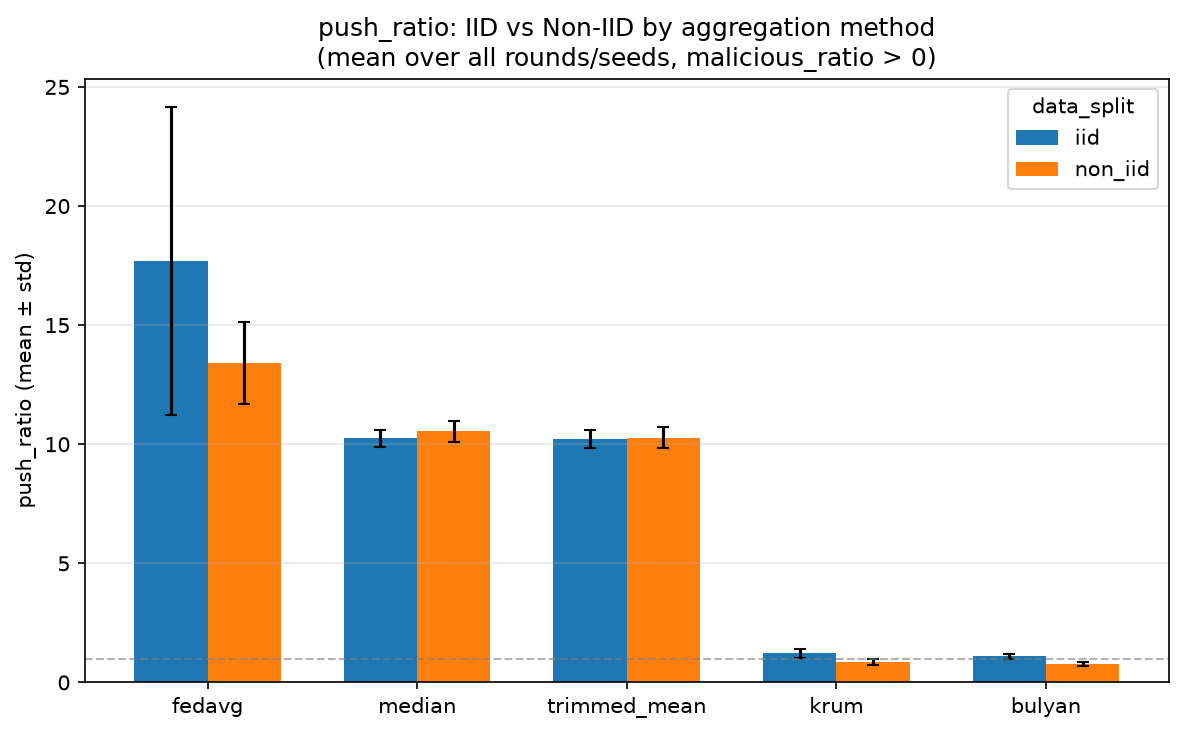
\includegraphics[width=\columnwidth]{experiments_phase1/analysis/push_ratio_iid_vs_noniid.png}
    \caption{push\_ratio の手法別・IID/Non-IID別比較（全ラウンド・全Seed平均，Malicious Ratio $>0$）}
    \label{fig:phase1_push_ratio}
\end{figure}

\subsubsection{Krum・BulyanにおけるMalicious Ratio 0.0時の精度変動の要因}
\label{sec:krum_bulyan_spread_analysis}

Malicious Ratio 0.0（悪性クライアント不在）条件下でのAccuracyとbenign\_spreadの推移を図\ref{fig:phase1_krum_iid_spread}--\ref{fig:phase1_bulyan_noniid_spread}に示す。学習初期（Round 5未満）を除いた定常状態（Round 5以降）でのRound間Accuracy変化量（絶対値平均）を比較すると，Krumは IID 0.0082 に対し Non-IID 0.0543（最大0.1564）と約6.6倍に拡大するのに対し，Bulyanは IID 0.0026，Non-IID 0.0029 とほぼ同水準で安定している。

benign\_spreadの推移自体は，Krum・Bulyanのどちらも学習が進むにつれて低下し，Round 5以降はほぼ横ばいで推移する点で共通している（図下段）。したがって，Krum Non-IIDにおける定常状態後もAccuracyが上下に振動し続ける現象は，benign\_spreadの大小そのものよりも，各ラウンドでKrumが選択する少数のクライアント（またはその更新）がラウンドごとに入れ替わり，Non-IID環境ではクライアントごとのローカルデータ分布が偏っているために選ばれるクライアントによってモデル品質が大きくばらつくこと，が主要因と考えられる。Bulyanは複数候補を集約してから外れ値を除去する多段構成であるため，単一に近い候補の選択に強く依存するKrumよりもこの影響を受けにくく，Non-IIDでも安定した挙動を示したと解釈できる。

\begin{figure}[H]
    \centering
    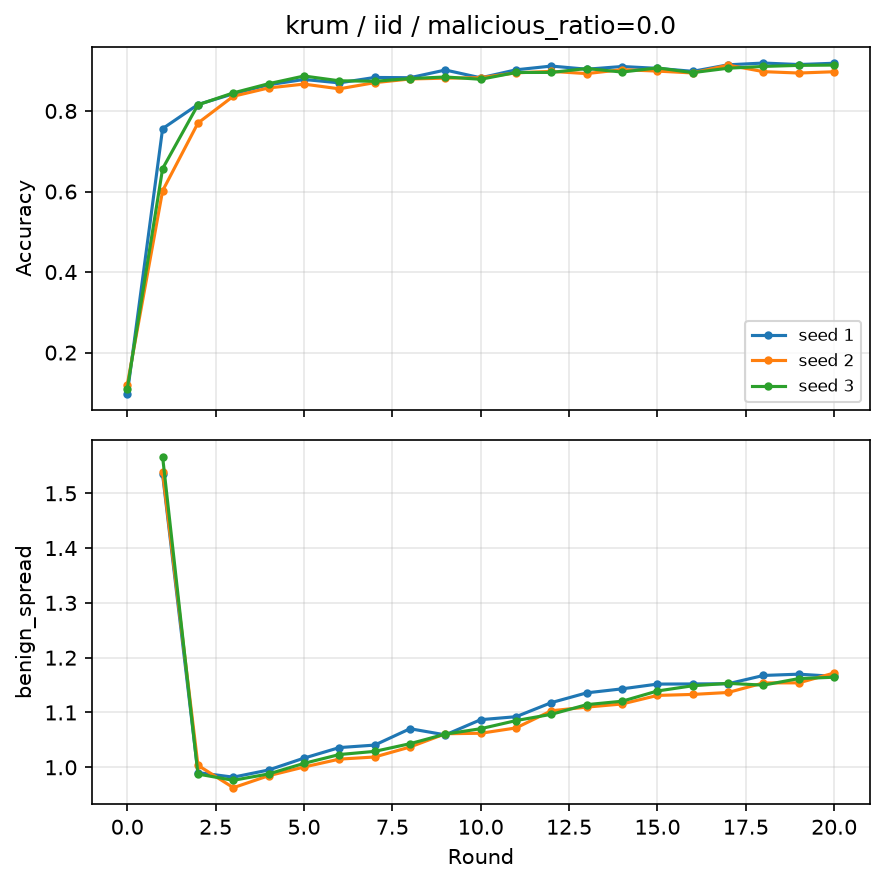
\includegraphics[width=\columnwidth]{experiments_phase1/analysis/krum_iid_ratio0.0_spread_vs_accuracy.png}
    \caption{Krum・IID・Malicious Ratio 0.0 におけるAccuracyとbenign\_spreadの推移（Seed別）}
    \label{fig:phase1_krum_iid_spread}
\end{figure}

\begin{figure}[H]
    \centering
    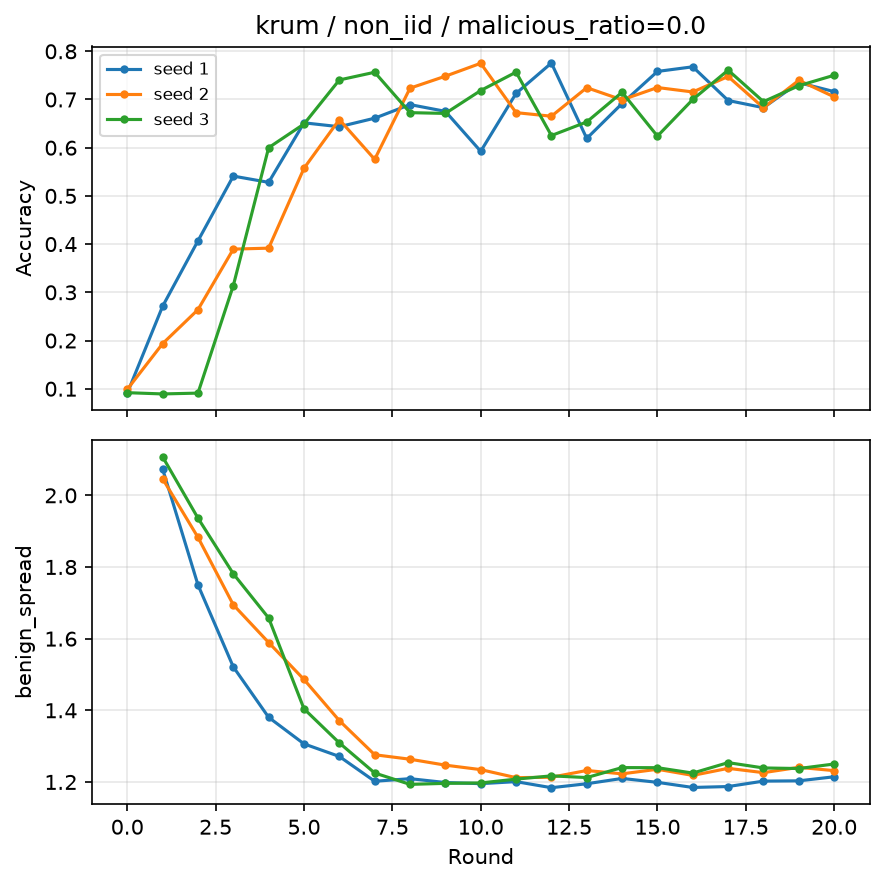
\includegraphics[width=\columnwidth]{experiments_phase1/analysis/krum_non_iid_ratio0.0_spread_vs_accuracy.png}
    \caption{Krum・Non-IID・Malicious Ratio 0.0 におけるAccuracyとbenign\_spreadの推移（Seed別）}
    \label{fig:phase1_krum_noniid_spread}
\end{figure}

\begin{figure}[H]
    \centering
    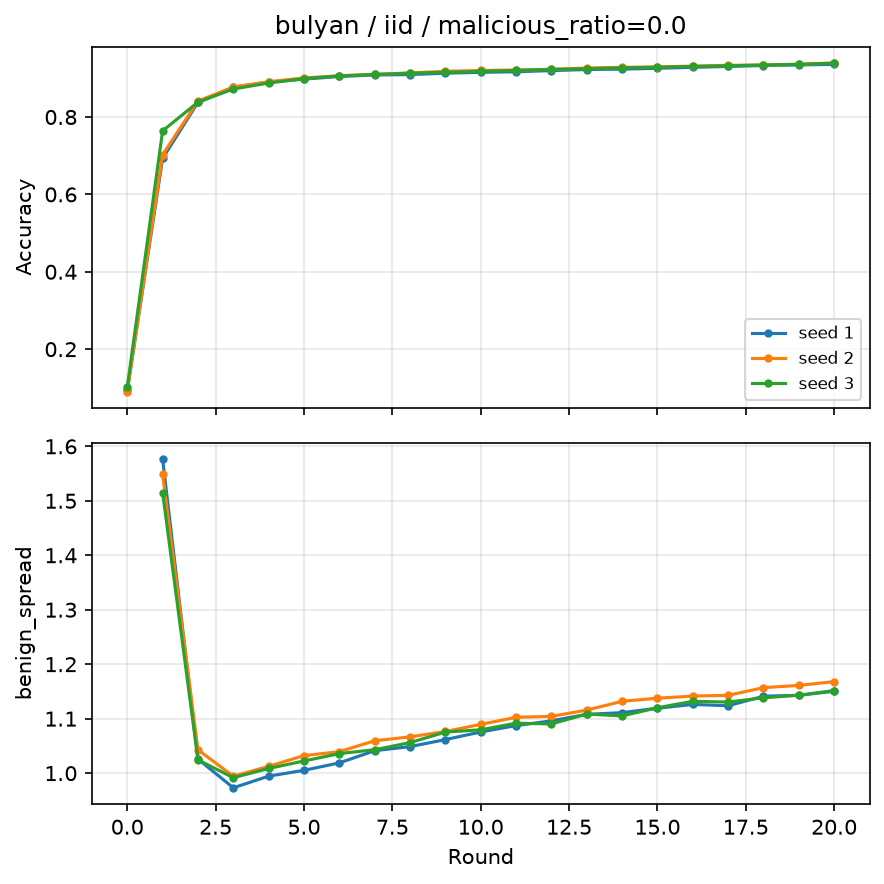
\includegraphics[width=\columnwidth]{experiments_phase1/analysis/bulyan_iid_ratio0.0_spread_vs_accuracy.png}
    \caption{Bulyan・IID・Malicious Ratio 0.0 におけるAccuracyとbenign\_spreadの推移（Seed別）}
    \label{fig:phase1_bulyan_iid_spread}
\end{figure}

\begin{figure}[H]
    \centering
    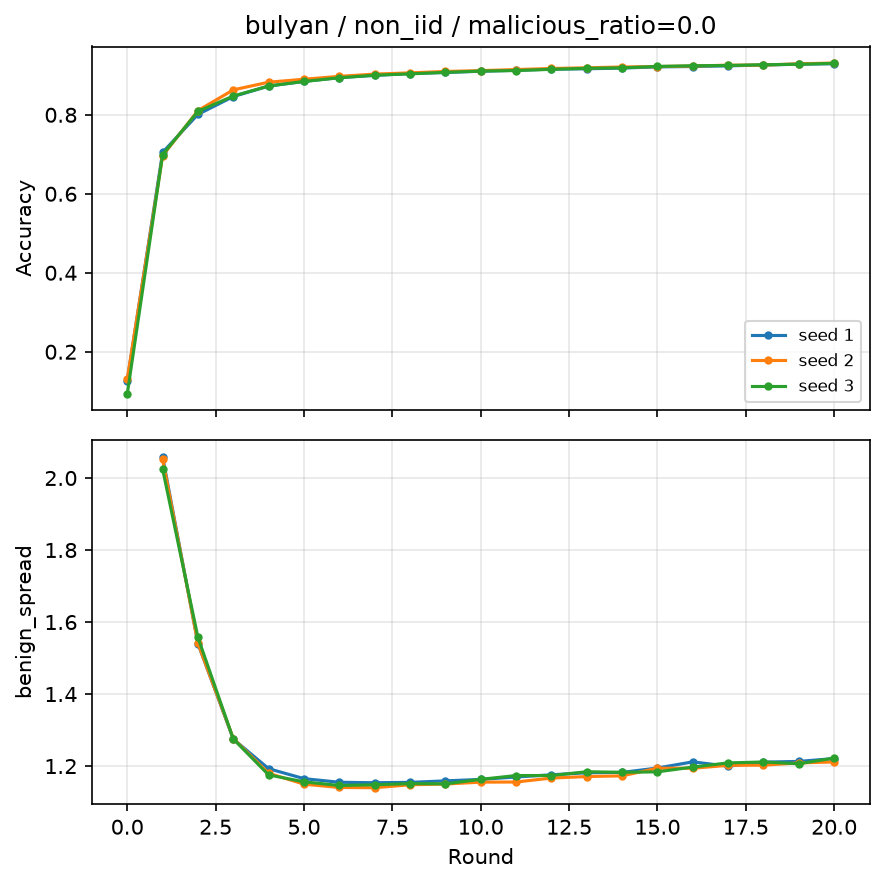
\includegraphics[width=\columnwidth]{experiments_phase1/analysis/bulyan_non_iid_ratio0.0_spread_vs_accuracy.png}
    \caption{Bulyan・Non-IID・Malicious Ratio 0.0 におけるAccuracyとbenign\_spreadの推移（Seed別）}
    \label{fig:phase1_bulyan_noniid_spread}
\end{figure}

\subsubsection{FedAvgにおける振動の定量化}

7.3節（既存実験）で定性的に観測されたFedAvgのRound間振動を，Round間Accuracy変化量（絶対値平均，IID/Non-IID・全Seed込み）で定量化した。Malicious Ratio 0.0では0.0431であるのに対し，Ratio 0.125で0.0837，Ratio 0.15--0.3では0.119前後まで拡大し，Ratio 0.0比で約2.8倍に達する。この振動幅の増大は，前項で述べたFedAvgのpush\_ratioの大きさ（選抜を経ないためmalicious更新のpushが抑制されない）と符合しており，Adaptive Model Poisoning Attackによる大きな更新ベクトルが単純平均に直接反映されることが振動の主因であるとの解釈を支持する。

\subsubsection{まとめとPhase 2への接続}

Phase 1の結果，計画時に想定していたTrimmed Mean（Non-IID，Ratio 0.3）に加え，KrumとFedAvgが広いRatio帯でSeed間ばらつきの主要因であることが明らかになった。特にKrum Non-IIDはRatio 0.3で攻撃の成否がSeedにより反転するレベルのばらつきを示しており，Phase 2ではこの23条件（表\ref{tab:phase1_seed_variance}および\texttt{seed\_variance.csv}参照）を対象にSeedを3から10へ増やし，ばらつきの統計的な安定性を検証する。

\subsection{Phase 2 実験結果}

\subsubsection{実行結果の概要}

Phase 1で特定した23条件それぞれについて，Seed 4--10の7本を追加実行した（計161回）。実行中に起動直後の一時的なログストリーム接続失敗が7件発生したが，いずれも再実行により正常終了しており，最終的な集計対象（\texttt{experiments\_phase2/\_logs/summary.csv}）に欠損はない。Phase 1のSeed 1--3とPhase 2のSeed 4--10を結合し，各条件についてSeed 10本での最終Accuracyの平均・標準偏差を再集計した（\texttt{experiments\_phase2/analyze\_combined.py}，出力は\texttt{combined\_analysis/}）。

\subsubsection{Seed数増加によるばらつきの再検証}

図\ref{fig:phase2_seed_variance_before_after}に，23条件それぞれについてSeed 3本時点（Phase 1のみ）とSeed 10本時点（Phase 1+2）の標準偏差を比較して示す。23条件中22条件で，Seed 10本に増やしてもしきい値0.02以上の高分散が維持された。上位10条件を表\ref{tab:phase2_seed_variance}に示す。

\begin{figure}[H]
    \centering
    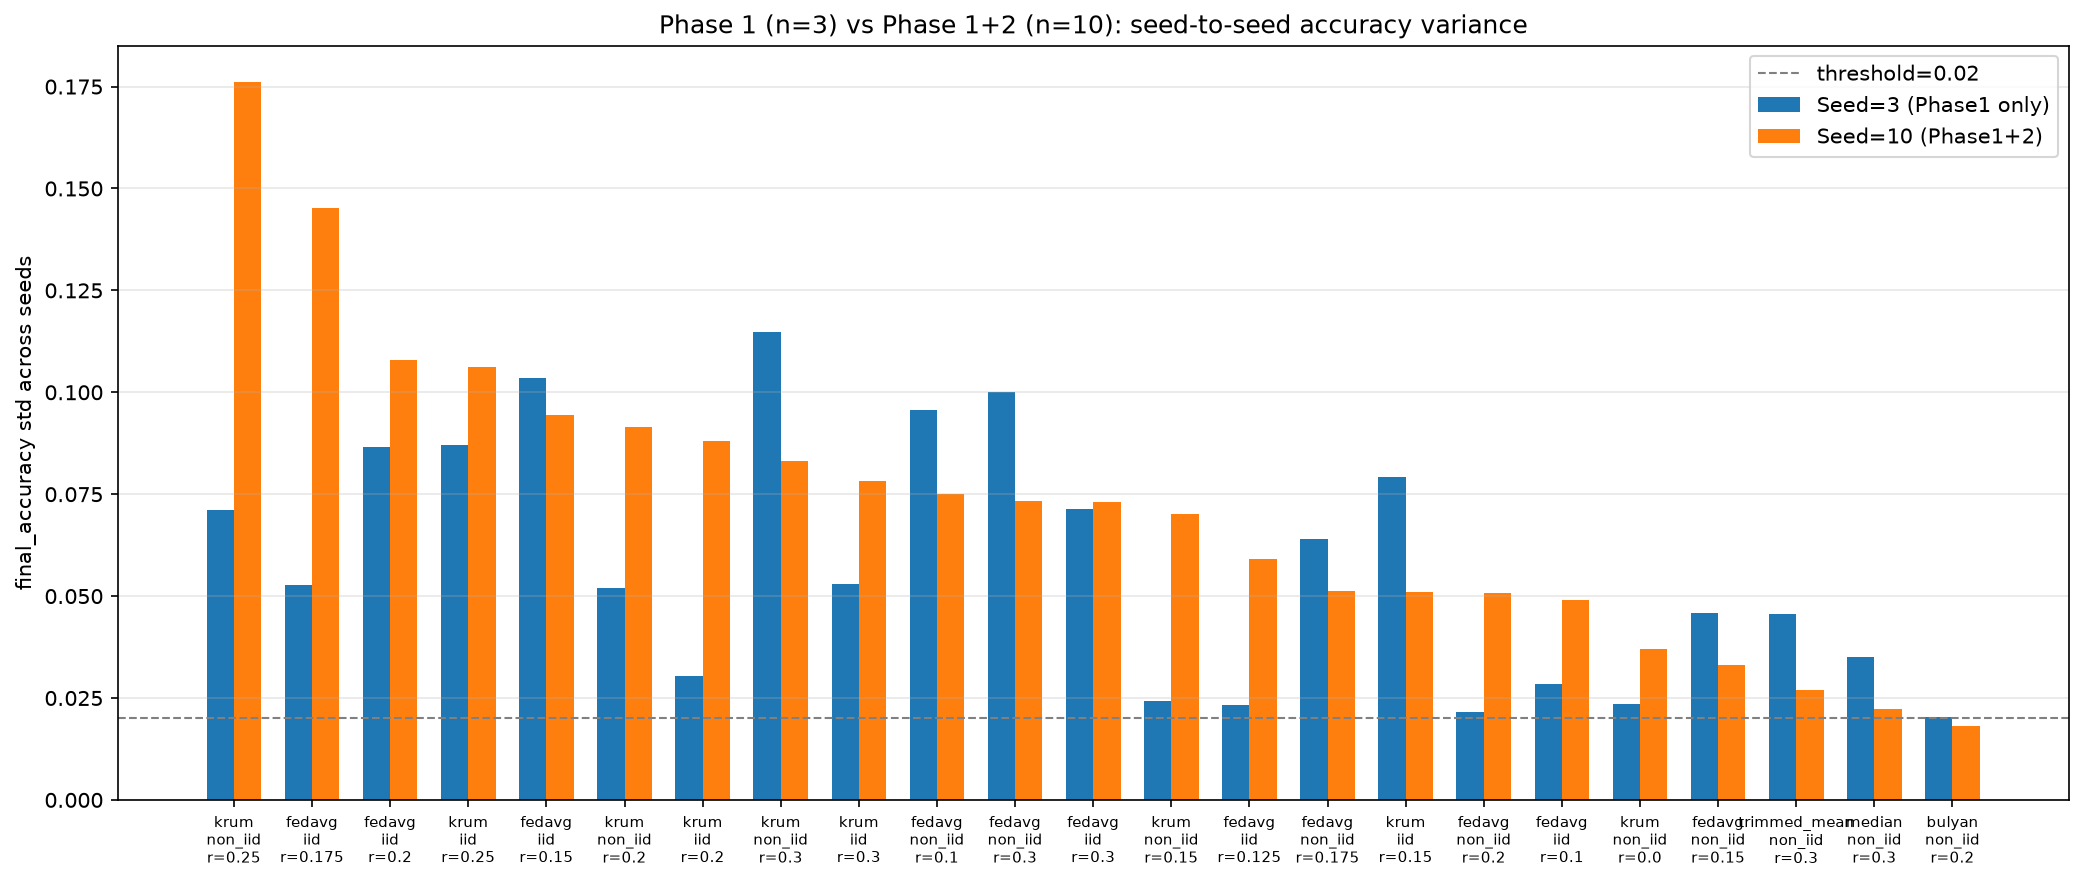
\includegraphics[width=\columnwidth]{experiments_phase2/combined_analysis/seed_variance_before_after.png}
    \caption{Phase 1（Seed 3本）と Phase 1+2（Seed 10本）における
    最終Accuracyの標準偏差の比較（acc\_std降順）}
    \label{fig:phase2_seed_variance_before_after}
\end{figure}

\begin{table}[H]
\centering
\caption{Seed 10本時点での標準偏差が大きい上位10条件}
\label{tab:phase2_seed_variance}
\footnotesize
\begin{tabular}{llccc}
\hline
手法 & 分布 & Ratio & std($n{=}3$) & std($n{=}10$) \\
\hline
Krum & Non-IID & 0.25 & 0.0711 & 0.1762 \\
FedAvg & IID & 0.175 & 0.0528 & 0.1451 \\
FedAvg & IID & 0.20 & 0.0865 & 0.1080 \\
Krum & IID & 0.25 & 0.0870 & 0.1063 \\
FedAvg & IID & 0.15 & 0.1036 & 0.0943 \\
Krum & Non-IID & 0.20 & 0.0520 & 0.0915 \\
Krum & IID & 0.20 & 0.0305 & 0.0881 \\
Krum & Non-IID & 0.30 & 0.1149 & 0.0832 \\
Krum & IID & 0.30 & 0.0531 & 0.0783 \\
FedAvg & Non-IID & 0.10 & 0.0957 & 0.0750 \\
\hline
\end{tabular}
\end{table}

特に顕著なのがKrum・Non-IID・Ratio 0.25であり，標準偏差はSeed 3本時点の0.0711からSeed 10本時点で0.1762へと約2.5倍に拡大し，10本のSeed間での最終Accuracyの範囲は0.129--0.600（幅0.471）に達した。図\ref{fig:phase2_krum_noniid_ratio025}に示すように，Phase 1のSeed 1--3（青）はいずれも比較的高い側（0.46--0.60）に偏っており，Phase 2で追加したSeed 4--10（橙）には0.13--0.32という低い値が複数含まれる。これは，Seed 3本による評価がこの条件の真の不安定性を過小評価していたことを意味する。同様にFedAvg・IID・Ratio 0.175でも標準偏差が0.0528から0.1451へとほぼ3倍に拡大し，最終Accuracyの範囲は0.381--0.760（幅0.379）に達した。

\begin{figure}[H]
    \centering
    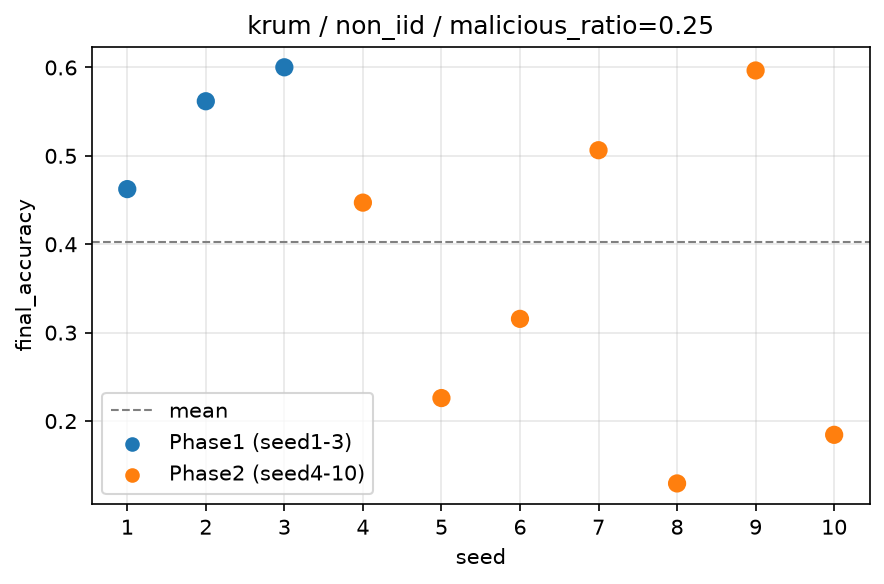
\includegraphics[width=\columnwidth]{experiments_phase2/combined_analysis/accuracy_by_seed_krum_non_iid_ratio0.25.png}
    \caption{Krum・Non-IID・Malicious Ratio 0.25 におけるSeed別最終Accuracy
    （青：Phase 1のSeed 1--3，橙：Phase 2のSeed 4--10）}
    \label{fig:phase2_krum_noniid_ratio025}
\end{figure}

23条件全体でSeed 10本時点の平均Accuracyを見ると，Seed 3本時点と比べて平均が上昇した条件が11件，低下した条件が12件とほぼ均等に分かれており，Phase 1のSeed選択が系統的に楽観・悲観いずれかに偏っていたわけではなく，単に3本という少ないSeed数では真のばらつきを捉えきれていなかったことを示している。

唯一しきい値を下回ったのはBulyan・Non-IID・Ratio 0.2であり，標準偏差はSeed 3本時点の0.0203からSeed 10本時点で0.0180へとわずかに減少した。図\ref{fig:phase2_bulyan_noniid_ratio02}に示すように，10本のSeedはいずれも0.805--0.855という狭い範囲に収まっており，Phase 1時点で既にしきい値付近であったこの条件は，Seed数を増やしても安定した挙動を示すことが確認された。すなわち，この条件については計画書2節で述べた「$n=3$での偶然の外れ値」ではなく，元々ばらつきの小さい条件がしきい値付近にあったに過ぎなかったと解釈できる。

\begin{figure}[H]
    \centering
    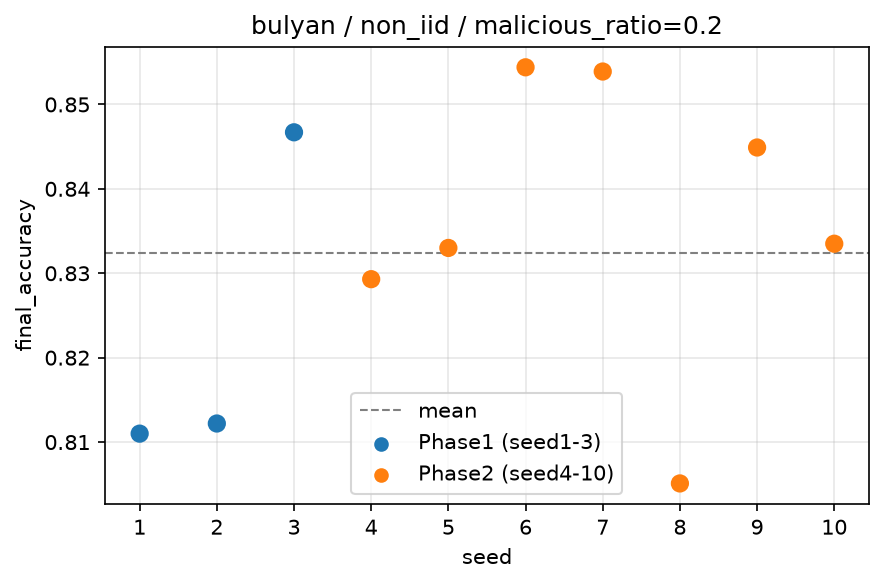
\includegraphics[width=\columnwidth]{experiments_phase2/combined_analysis/accuracy_by_seed_bulyan_non_iid_ratio0.2.png}
    \caption{Bulyan・Non-IID・Malicious Ratio 0.2 におけるSeed別最終Accuracy
    （青：Phase 1のSeed 1--3，橙：Phase 2のSeed 4--10）}
    \label{fig:phase2_bulyan_noniid_ratio02}
\end{figure}

\subsubsection{まとめ}

Phase 2の結果，Phase 1でSeed間ばらつきが大きいと判定された23条件のうち22条件（96\%）が，Seedを3本から10本に増やしても高分散のまま残ることが確認された。これは，\ref{sec:phase1_results}節で観測されたSeed間ばらつきの大半が，少数Seedによる評価の偶然の産物ではなく，KrumおよびFedAvgが中～高Malicious Ratio域で本質的に抱える不安定性であることを裏付けている。特にKrum・Non-IIDではRatio 0.25においてSeedによって最終Accuracyが0.13から0.60まで変動しており，単一または少数のSeedによる評価では攻撃の成否を正しく判定できないことが定量的に示された。一方，Bulyanは実行可能なRatio範囲においてSeed数を増やしても一貫して狭いばらつきに収まっており，KrumやFedAvgとは対照的な安定性を示した。

\begin{thebibliography}{99}

\bibitem{mammen2021fl}
Priyanka Mary Mammen,
``Federated Learning: Opportunities and Challenges,''
Proceedings of ACM Conference,
2021.
\bibitem{li2019fl}
Tian Li,
Anit Kumar Sahu,
Ameet Talwalkar,
Virginia Smith,
``Federated Learning: Challenges, Methods, and Future Directions,''
arXiv preprint arXiv:1908.07873,
2019.
\bibitem{ma2020privacy}
Chuan Ma,
Jun Li,
Ming Ding,
Howard H. Yang,
Feng Shu,
Tony Q. S. Quek,
H. Vincent Poor,
``On Safeguarding Privacy and Security in the Framework of Federated Learning,''
arXiv preprint arXiv:1909.06512,
2020.

\bibitem{sagar2023survey}
Subhash Sagar,
Chang-Tsun Li,
Seng W. Loke,
Jinho Choi,
``Poisoning Attacks and Defenses in Federated Learning: A Survey,''
IEEE Security \& Privacy,
2023.

\bibitem{fang2020local}
Minghong Fang,
Xiaoyu Cao,
Jinyuan Jia,
Neil Zhenqiang Gong,
``Local Model Poisoning Attacks to Byzantine-Robust Federated Learning,''
Proceedings of the 29th USENIX Security Symposium (USENIX Security 2020),
pp. 1605--1622,
2020.
\bibitem{mcmahan2017fedavg}
H. Brendan McMahan,
Eider Moore,
Daniel Ramage,
Seth Hampson,
Blaise Aguera y Arcas,
``Communication-Efficient Learning of Deep Networks from Decentralized Data,''
Proceedings of the 20th International Conference on Artificial Intelligence and Statistics (AISTATS),
pp. 1273--1282,
2017.
\bibitem{xie2020dba}
Chulin Xie,
Keli Huang,
Pin-Yu Chen,
Bo Li,
``DBA: Distributed Backdoor Attacks against Federated Learning,''
International Conference on Learning Representations (ICLR),
2020.
\bibitem{nguyen2022flame}
Tuan D. Nguyen et al.,
``FLAME: Taming Backdoors in Federated Learning,''
31st USENIX Security Symposium (USENIX Security 2022),
pp. 1415--1432,
2022.
\bibitem{bagdasaryan2020model}
Eugene Bagdasaryan,
Andreas Veit,
Yiqing Hua,
Deborah Estrin,
Vitaly Shmatikov,
``How To Backdoor Federated Learning,''
Proceedings of the 23rd International Conference on Artificial Intelligence and Statistics (AISTATS),
pp. 2938--2948,
2020.
\end{thebibliography}


\end{document}